\documentclass{article}
\usepackage[utf8]{inputenc}
\usepackage[spanish]{babel}
\usepackage{listings}
\usepackage{subfigure}
\usepackage{graphicx}
\usepackage{url}
\usepackage{multirow}
\usepackage{color}
\usepackage{booktabs}
\usepackage{float}
\usepackage{amsmath}
\usepackage{hyperref}
\hypersetup{
    colorlinks=true,
    linkcolor=blue,
    filecolor=magenta,      
    urlcolor=cyan,
}
\usepackage[margin=3cm,twoside]{geometry} 
\setlength{\parindent}{0pt}
\setlength{\parskip}{1em}


\definecolor{mygreen}{rgb}{0,0.6,0}
\definecolor{mygray}{rgb}{0.5,0.5,0.5}
\definecolor{mymauve}{rgb}{0.58,0,0.82}
\lstset{ 
  backgroundcolor=\color{white},   % choose the background color; you must add \usepackage{color} or \usepackage{xcolor}; should come as last argument
  basicstyle=\footnotesize,        % the size of the fonts that are used for the code
  breakatwhitespace=false,         % sets if automatic breaks should only happen at whitespace
  breaklines=true,                 % sets automatic line breaking
  captionpos=b,                    % sets the caption-position to bottom
  commentstyle=\color{mygreen},    % comment style
  deletekeywords={...},            % if you want to delete keywords from the given language
  escapeinside={\%*}{)},          % if you want to add LaTeX within your code
  extendedchars=true,              % lets you use non-ASCII characters; for 8-bits encodings only, does not work with UTF-8
  firstnumber=1,                % start line enumeration with line 1000
  frame=single,	                   % adds a frame around the code
  keepspaces=true,                 % keeps spaces in text, useful for keeping indentation of code (possibly needs columns=flexible)
  keywordstyle=\color{blue},       % keyword style
  language=Octave,                 % the language of the code
  morekeywords={*,...},            % if you want to add more keywords to the set
  numbers=left,                    % where to put the line-numbers; possible values are (none, left, right)
  numbersep=5pt,                   % how far the line-numbers are from the code
  numberstyle=\tiny\color{mygray}, % the style that is used for the line-numbers
  rulecolor=\color{black},         % if not set, the frame-color may be changed on line-breaks within not-black text (e.g. comments (green here))
  showspaces=false,                % show spaces everywhere adding particular underscores; it overrides 'showstringspaces'
  showstringspaces=false,          % underline spaces within strings only
  showtabs=false,                  % show tabs within strings adding particular underscores
  stepnumber=1,                    % the step between two line-numbers. If it's 1, each line will be numbered
  stringstyle=\color{mymauve},     % string literal style
  tabsize=2,	                   % sets default tabsize to 2 spaces
  title=\lstname                  % show the filename of files included with \lstinputlisting; also try caption instead of title
}
\usepackage{etoolbox}
\makeatletter
\providecommand{\subtitle}[1]{% add subtitle to \maketitle
  \apptocmd{\@title}{\par {\large #1 \par}}{}{}
}
\renewcommand{\theenumi}{\roman{enumi}}
\newtheorem{teor}{Teorema}
\makeatother
\title{Tarea 6 de Modelos Probabilistas Aplicados}
\subtitle{Algoritmos generadores de números pseudo-aleatorios con distribución Uniforme y distribución Normal}

\author{5271}
\date{\today}

\begin{document}

\maketitle

\section{Introducción}

En este trabajo se presenta un acercamiento al tema pruebas estadísticas, dando respuestas a una serie de preguntas que dan cuerpo a una breve introducción en dicho tema. Además se realizan diversas pruebas estadísticas como ejemplos. Los datos que se utilizan en este trabajo fueros obtenidos en el sitio \href{https://www.inegi.org.mx/default.html}{https://www.inegi.org.mx} que pertenece al Instituto Nacional de Estadística y Geografía (INEGI). Se escogió el apartado Construcción donde se muestra información sobre los principales resultados de las Empresas Constructoras, comprende unidades económicas dedicadas principalmente a la edificación; a la construcción de obras de ingeniería civil y a la realización de trabajos especializados de construcción. De este apartado se descargó el tabulado (Valor de producción generado por las empresas constructoras según el tipo de obra) en formato \textit{csv}. Las pruebas se  realizan en el programa R versión 4.0.2 \cite{r} en el entorno de desarrollo Rstudio \cite{rstudio}

\section{Pruebas estadísticas}
En esta sección se realiza un acercamiento a temas importantes relacionados con las pruebas estadísticas, como su características generales, los tipos de pruebas e interpretación de las mismas. 

\subsection{Relación entre contraste de hipótesis y pruebas estadísticas}
\label{sec:1}
Una prueba estadística un procedimiento en el cual se analiza la evidencia proporcionada por los datos con el fin de probar una Hipótesis.La hipótesis estadística es una afirmación sobre los valores del parámetro $\theta$ ($\theta$ puede ser: $\mu$, $p$, $\sigma^{2}$, entre otros) de una población o proceso, que es susceptible de probarse a partir de la información contenida en una muestra representativa que es obtenida de la población. Trasladando esto al tema de investigación del autor (Empaquetamiento óptimo), se tiene el siguiente ejemplo, la afirmación ``Existe diferencia en el porciento de ocupación  de los diferentes tipos de figuras en el contenedor". La veracidad de esta afirmación se obtiene al contrastar las siguientes hipótesis:
\begin{equation}\label{eq:1}
H_{0}:\mu_{1}=\mu_{2}=\mu_{3}=\mu_{4}=\mu_{5}=\mu_{6},    
\end{equation}
\begin{equation}\label{eq:2}
 H_{1}:\mu_{i}\neq\mu_{j}\quad para\quad alguna \quad i\neq j.
\end{equation}
A la expresión (\ref{eq:1}) se le conoce como hipótesis nula y a la expresión (\ref{eq:2}) se le nombra como hipótesis alternativa. El nombre de hipótesis nula nace de que comúnmente se plantea como una igualdad. Generalmente se trata de probar que la hipótesis nula es verdadera, y que en caso de ser rechazada por la evidencia que aportan los datos, se aceptará la hipótesis alternativa.

En el cuadro \ref{tab:1} de la página \pageref{tab:1} se muestra el resultado de la aplicación de un análisis de varianza (ANOVA) al ejemplo antes mencionado. Con los valores del estadístico de prueba \textbf{F} = 1.0302 y el \textbf{valor p} = 0.4117, se tiene evidencia para aceptar la hipótesis $H_{0}$, la cual indica que no existe diferencias estadísticas significativas entre los tratamientos con un intervalo de confianza del $95\%$. Esto se puede observar en la figura \ref{fig:1} de la de la página \pageref{fig:1}.  

\begin{table}
  \centering
  \caption{Influencia del tipo de figura en el \% de ocupación del contenedor}
 
    \begin{tabular}{clrrrrrr}
    \toprule
          & \textbf{Factor} & \multicolumn{1}{l}{\textbf{SS}} & \multicolumn{1}{l}{\textbf{DF}} & \multicolumn{1}{l}{\textbf{MS}} & \multicolumn{1}{l}{\textbf{F}} & \multicolumn{1}{l}{\textbf{Valor p}} & \multicolumn{1}{l}{\textbf{np2}} \\
    \midrule
    0     & Tipo de figura & 0.0132 & 5.0000     & 0.0026 & 1.0302 & 0.4147 & 0.1252 \\
    1     & Within & 0.0920 & 36.0000    & 0.0026 &       &       &  \\
    \bottomrule
    \end{tabular}%

    \label{tab:1}
\end{table}
    
 \begin{figure}
    \centering
    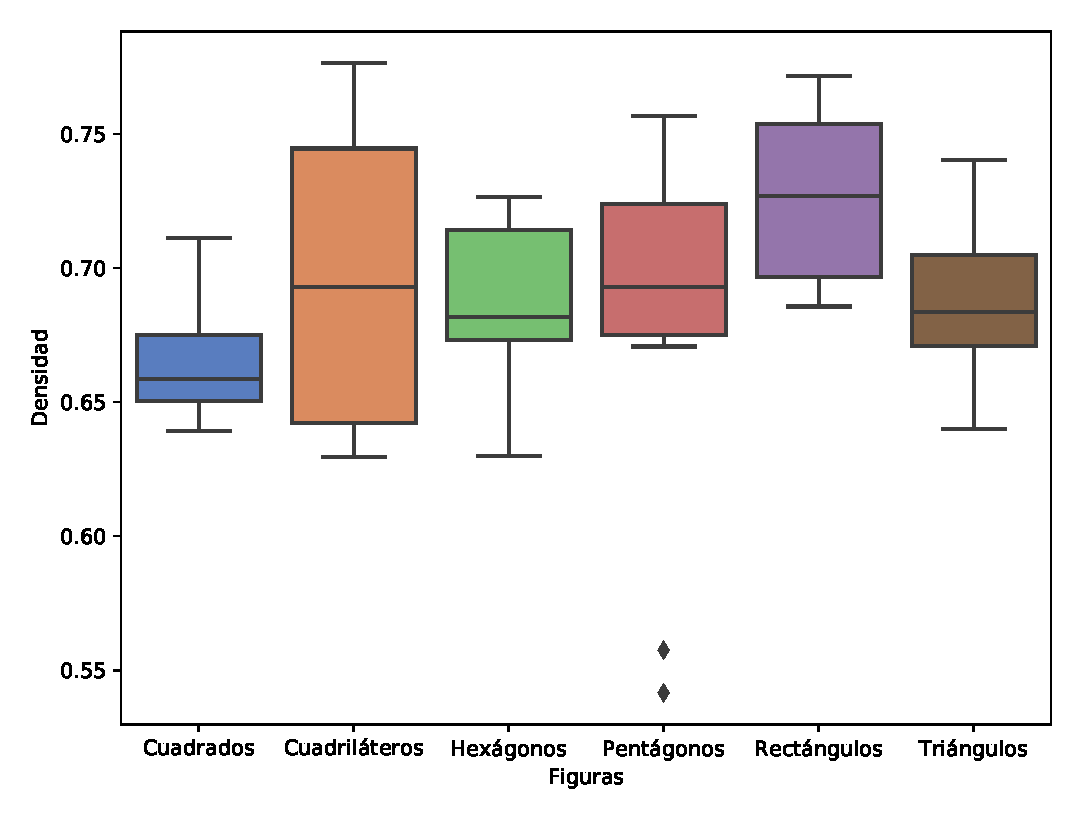
\includegraphics[scale=0.8]{figuras/boxplot_Figuras.eps}
    \caption{Diagrama de caja y bigotes que relaciona los tipos de figuras y el \% de ocupación del contenedor.}
    \label{fig:1}
\end{figure}


\subsection{En que casos se rechaza la hipótesis nula}
\label{sec:2}
Para probar una hipótesis se trata de corroborar que la afirmación planteada por la hipótesis nula ($H_{0}$) es verdad o no. Se parte del supuesto que  es verdadera, si la evidencia arrojada por los datos es suficiente para contradecir dicho supuesto se rechaza $H_{0}$ y se acepta la Hipótesis alternativa ($H_{1}$). En caso de no haber evidencias suficientes que demuestren la falsedad de la $H_{0}$ esta no se rechaza, es decir $H_{0}$ es verdad hasta que no se demuestre lo contrario.

Para discernir si $H_{0}$ se rechaza o no, se utiliza un estadístico de prueba el cual es un es un número calculado a partir de los datos y la hipótesis nula. Al conjunto de posibles valores del estadístico de prueba que llevan a rechazar $H_{0}$, se le llama región o intervalo de rechazo para la prueba, y a los posibles valores donde no se rechaza $H_{0}$ se les conoce como región o intervalo de confianza.

El estadístico de prueba, construido bajo el supuesto de que $H_{0}$ es verdad, es una variable aleatoria con distribución conocida. Si efectivamente $H_{0}$ es verdad, el valor del estadístico de prueba debería caer dentro del rango de valores más probables de su distribución asociada, el cual se conoce como región de confianza. Si cae en una de las colas de su distribución asociada, fuera del rango de valores más probables (en la región de rechazo), es evidencia en contra de que este valor pertenece a dicha distribución. De aquí se deduce que debe estar mal el supuesto bajo el cual se construyó, es decir, H0 debe ser falsa \cite{}.

Análogamente al análisis del ejemplo de la sección \ref{sec:1}, se realiza la misma prueba para el factor de control cantidad de figuras. Obtenemos como resultado el cuadro \ref{tab:2} de la página \pageref{tab:2}. Con los valores del estadístico de prueba \textbf{F} = 4.9514 y con un \textbf{valor p} = 0.0015 menor que 0.05, se tiene evidencia para rechazar la hipótesis $H_{0}$ ya que existe diferencias estadísticas significativas al menos entre algunos de los grupos con un intervalo de confianza de un $\textbf{95\%}$ como se muestra en la figura \ref{fig:2} de la página \pageref{fig:2}.

\begin{table}
  \centering
  \caption{Influencia de la cantidad de figura en el \% de ocupación del contenedor}
    \begin{tabular}{clrrrrrr}
    \toprule
          & \textbf{Factor} & \textbf{SS} & \textbf{DF} & \textbf{MS} & \textbf{F} & \textbf{Valor p} & \textbf{np2} \\
    \midrule
    0     & Cantidad defiguras & 0.0429 & 5.0000 & 0.0086 & 4.9514 & 0.0015 & 0.4075 \\
    1     & Within & 0.0623 & 36.0000 & 0.0017 & -- & -- & -- \\
    \bottomrule
    \end{tabular}%
  \label{tab:2}%
\end{table}%
\begin{figure}
    \centering
    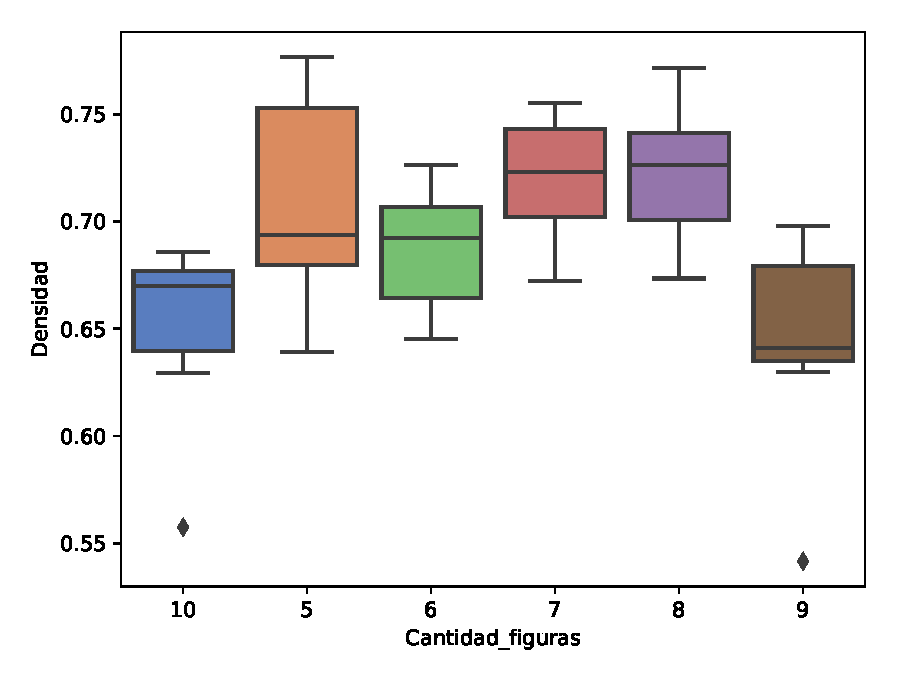
\includegraphics[scale=0.8]{figuras/boxplot_Cantidad_figuras.eps}
    \caption{Diagrama de caja y bigotes que relaciona los cantidad de figuras y el \% de ocupación del contenedor.}
    \label{fig:2}
\end{figure}

\subsection{Interpretación de la salida de una prueba estadística}
\label{sec:3}
 En la sección \ref{sec:1} y \ref{sec:2}  muestran ejemplos de como interpretar la salidas de las pruebas estadísticas a través de los estadísticos de prueba explicados en la sección \ref{sec:2} y el \textbf{valor p}, representa una probabilidad que mide la evidencia en contra de la hipótesis nula. \textbf{valor p} más pequeño proporciona una evidencia más fuerte en contra de la hipótesis nula.
 
 Para determinar si la diferencia entre las desviaciones estándar o las varianzas de las poblaciones es estadísticamente significativa, se compara el \textbf{valor p} con el nivel de significancia. Por lo general, el nivel de significancia (denotado como $\alpha$) indica el riesgo de concluir que existe una diferencia cuando realmente no la hay.
 \begin{itemize}
   \item Sí el \textbf{valor p} $> \alpha $, la relación de las desviaciones estándar o las varianzas no es estadísticamente significativa (no puede rechazar $H_{0}$).
   
     \item Sí el \textbf{valor p} $\leq \alpha $, la relación de las desviaciones estándar o las varianzas es estadísticamente significativa (se rechaza $H_{0}$).
   
 \end{itemize}
 
 

\subsection{Selección de nivel de significancia}
\label{sec:4}
El valor de $\alpha$ es el máximo nivel de riesgo aceptable de rechazar la hipótesis nula cuando la hipótesis nula es verdadera, como se comento en la sección \ref{sec:3}. Por lo general, se elige elige el nivel de significancia antes de analizar los datos. El este nivel se calcula como 1 menos el intervalo de confianza. Para los ejemplos anteriores se empleo un intervalo de confianza del 95\%, por lo que $\alpha$ es igual a 0.05.

Los valores de $\alpha$ son elegidos en dependencia de la finalidad de la prueba, es decir si se quiere determinar cualquier diferencia que exista se utiliza un valor de $\alpha$ mas grande (0.10). En el caso que se quiera asegurar que el las diferencias que existen son reales, se emplea un valor de $\alpha$ muy pequeño (0.01). Comúnmente se utiliza el valor de $\alpha$ igual a 0.05. 

\subsection{Errores frecuentes de interpretación del \textbf{valor p}}
\label{sec:5}

Probar una hipótesis estadística es una decisión probabilística, por lo que existe el
riesgo de cometer un error \textbf{tipo I} o un error \textbf{tipo II}. El primero ocurre cuando se rechaza $H_{0}$ cuando ésta es verdadera, y el error \textbf{tipo II} es cuando se acepta $H_{0}$ y ésta es falsa. Con $\alpha$ y $\beta$ se denotan las probabilidades de los errores \textbf{tipo I} y \textbf{tipo II}, respectivamente.

Donde $\alpha$ es el nivel de significancia explicado en la sección \ref{sec:4}. Y $\beta$ es la llamada potencia de prueba.

\subsection{Potencia de prueba, utilidad}
\label{sec:6}
A 1 – $\beta$ se le llama potencia de la prueba, y es la probabilidad de rechazar $H_{0}$
cuando es falsa. Por lo general, en las pruebas de hipótesis se especifica el valor de $\alpha$ y se diseña la prueba de tal forma que el valor de $\beta$ sea pequeño. Esto es, la probabilidad del error \textbf{tipo I} se controla directamente, mientras que la probabilidad de error \textbf{tipo II} se controla de manera indirecta con el tamaño de la muestra, ya que a más datos $\beta$ será menor. Es decir, con una muestra grande es mayor la potencia de la prueba, de manera que se incrementa la probabilidad de rechazar $H_{0}$ si ésta es falsa.

\subsection{Pruebas paramétricas}
\label{sec:7}

Para la aplicación de las pruebas paramétricas, los datos deben cumplir ciertas presunciones:
\begin{itemize}
    \item Los datos son de escala de intervalo o razón.
    \item La población de la muestra debe aproximarse a una distribución normal.
    \item Las varianzas de las muestras deben aproximadamente similares.
    \item Las observaciones deben ser independientes entre sí.
\end{itemize}
Entre las pruebas perimétricas más usadas están: 
\begin{itemize}
\item Prueba de Shapiro-Wilks.
\item Prueba de Fisher.
\item Prueba t de Student para muestras independientes.
\item Coeficiente de correlación de Pearson.
\item Regresión lineal.
\item Análisis de varianza factorial (ANOVA).
\item Análisis de covarianza (ANCOVA).
\end{itemize}
 En ambos ejemplos presentados en la sección \ref{sec:1} y \ref{sec:2} Antes de realizar el ANOVA, se realiza la prueba de Shapiro-Wilk, que calcula un W estadístico que prueba si una muestra aleatoria $x_{1},x_{2},...,x_{n}$ proviene de una distribución normal. El resultado de esta prueba se muestra en el cuadro \ref{tab:3} de la página \pageref{tab:3}. En dicho cuadro con un \textbf{W} = 0.9537  y un  \textbf{valor p} = 0.0877 mayor que 0.05, se puede observar que la variable dependiente (\% de ocupación) sigue una distribución normal con un intervalo de confianza del 95\%.

\begin{table}
  \centering
  \caption{Prueba Shapiro-Wilk a la variable \% de ocupación}
  \resizebox{6cm}{!}{
    \begin{tabular}{ccc}
    \toprule
          & \textbf{W} & \textbf{Valor p }  \\
    \midrule
    \% de ocupación & 0.9537 & 0.0877  \\
    \bottomrule
    \end{tabular}%
    }
  \label{tab:3}%
\end{table}%

\subsection{Pruebas no paramétricas}
\label{sec:8}
En la sección \ref{sec:7} se plantea características que deben tener los datos para usar las pruebas paramétricas. Cuando los datos no cumplen una de estas características. Se emplean las pruebas no paramétricas, ejemplos de estas son:
\begin{itemize}
    \item Prueba Chi-cuadrada.
    \item Coeficientes de correlación e independencia para tabulaciones cruzadas.
    \item Coeficientes de correlación por rangos ordenados Spearman y Kendall.
    \item Prueba  H  de  Kruskal-Wallis.  
\end{itemize}

Como en los ejemplos anteriores se realiza una prueba de Shapiro-Wilk para corroborar que la variable dependiente (\% de ocupación) variando el tipo de contenedor, sigue una distribución normal. Los resultados obtenidos con un \textbf{W} = 0.9528 y \textbf{valor p}=0.0038 menor que 0.05, nos muestra que dicha variable no sigue una distribución normal con un intervalo de confianza del \textbf{95\%}. Lo antes expuestos se puede observar en la cuadro \ref{tab:4} de la página \pageref{tab:4}.

% Table generated by Excel2LaTeX from sheet 'normal'
\begin{table}
  \centering
  \caption{Prueba Shapiro-Wilk a la variable \% de ocupación variando el contenedor}
    \begin{tabular}{lrrl}
    \toprule
          & \textbf{W} & \textbf{Valor p} & \textbf{Normal} \\
    \midrule
    Densidad & 0.9527 & 0.0037& Falso  \\
    \bottomrule
    \end{tabular}%
  \label{tab:4}%
\end{table}%


Dado que los valores de la variable dependiente no sigue una distribución normal, se aplica la prueba H de Kruskal-Wallis que es una versión no paramétrica de ANOVA. En este caso se plantea la afirmación: ``Existen diferencias en el \% de ocupación según el tipo de contenedor".

Según los datos obtenidos en la prueba que se muestran en el cuadro \ref{tab:5} de la página \pageref{tab:5}. Estos resultados con un valor del estadístico de prueba \textbf{H} = 13.9167 y \textbf{valor p} = 0.0002, se rechaza la hipótesis $H_{0}$ aceptando la $H_{1}$, la cual indica que existen diferencias estadísticamente significativas entre los tipos de contenedores. En esta ocasión con los resultados de la prueba H de Kruskal-Wallis son suficientes para asegurar lo anterior dado que solo son dos los tipos de contenedores analizados. Gráficamente se puede observar esta conclusión en la figura \ref{fig:3} de la página \pageref{fig:3}.

% Table generated by Excel2LaTeX from sheet 'krukal'
\begin{table}
  \centering
  \caption{Prueba H de Kruskal-Wallis que relaciona el \% de ocupación con el tipo de contenedor }
    \begin{tabular}{ccccc}
    \toprule
          & \textbf{Factor} & \textbf{ddof1} & \textbf{H} & \textbf{pval} \\
    \midrule
    Kruskal & Contenedor & 1.0000 & 13.9167 & 0.0002 \\
    \bottomrule
    \end{tabular}%
  \label{tab:5}%
\end{table}%

\begin{figure}
    \centering
    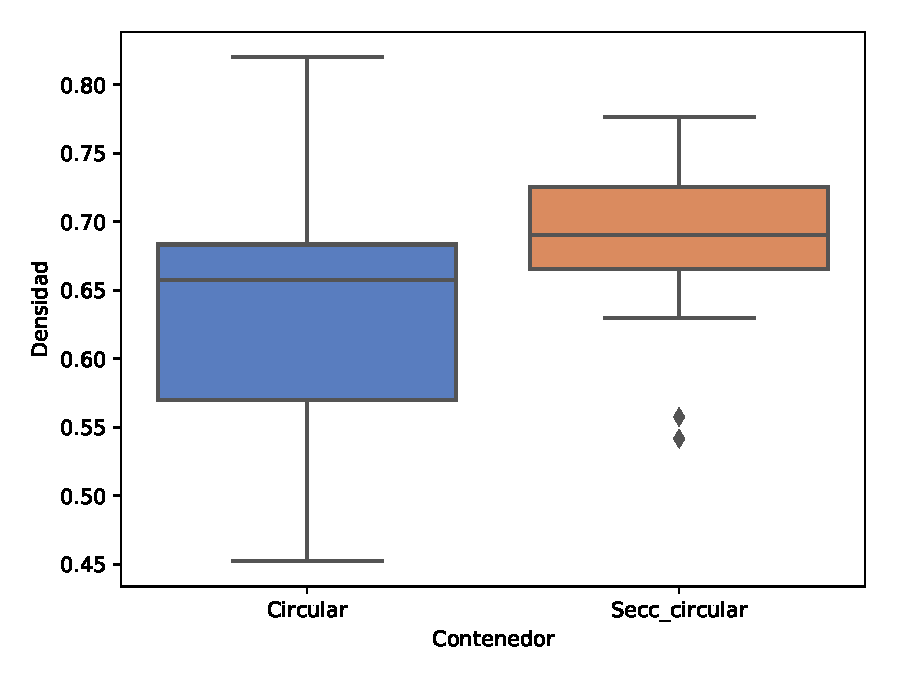
\includegraphics[scale=0.7]{figuras/boxplot_Contenedor.eps}
    \caption{Diagrama de caja y bigotes que relaciona los tipos de contenedor y el \% de ocupación del mismo.}
    \label{fig:3}
\end{figure}

\section{Aplicación de Pruebas estadísticas}

En esta sección se presentaran diversas pruebas estadísticas aplicas a los datos del sector de la construcción obtenidos de INEGI.

\subsection{Prueba de Shapiro-Wilk}
\label{sec:9}
Como se explica en la sección \ref{sec:7} la prueba de Shapiro-Wilk se utiliza para probar si los datos siguen una distribución normal. Por lo cual esta prueba es la primera que se le realiza a los datos para conocer la naturaleza de los mismo y así elegir el tipo de prueba a utilizar. Para el caso de ejemplo se tomara los valores de producción de las constructoras según el tipo de obras. En el cuadro \ref{tab:6} de la página \pageref{tab:6} se muestra obtenidos en las pruebas. Además la figura \ref{fig:4} de la página \pageref{fig:4} muestra como se comportan los datos según el tipo de obra.  

Las pruebas se realizan con un $\alpha$ = 0.05, y la hipótesis planteada es la siguiente: 
\begin{equation}\label{eq:1}
H_{0}:\text{La muestra sigue un distribución igual a la normal},    
\end{equation}
\begin{equation}\label{eq:2}
 H_{1}:\text{La muestra sigue un distribución diferente a la normal}. 
\end{equation}


% Table generated by Excel2LaTeX from sheet 'Hoja1'
\begin{table}
  \centering
  \caption{Resultados de la prueba de Shapiro-Wilk}
    \begin{tabular}{lrrl}
    \toprule
    \multicolumn{1}{c}{\textbf{Tipo de obra}} & \multicolumn{1}{c}{\textbf{W}} & \multicolumn{1}{c}{\textbf{Valor p}} &  \\
    \midrule
    \textbf{Agua, riego y saneamiento} & 0.9907 & 0.3223 &        $>\alpha$  \\
    \textbf{Petróleo y petroquímica} & 0.9659 & 0.0002 &      $<\alpha$ \\
    \textbf{Otras construcciones} & 0.9451 & 0.0000 &       $<\alpha$ \\
    \bottomrule
    \end{tabular}%
  \label{tab:6}%
\end{table}%

\begin{figure}
\centering
\subfigure[Agua, riego y saneamiento]{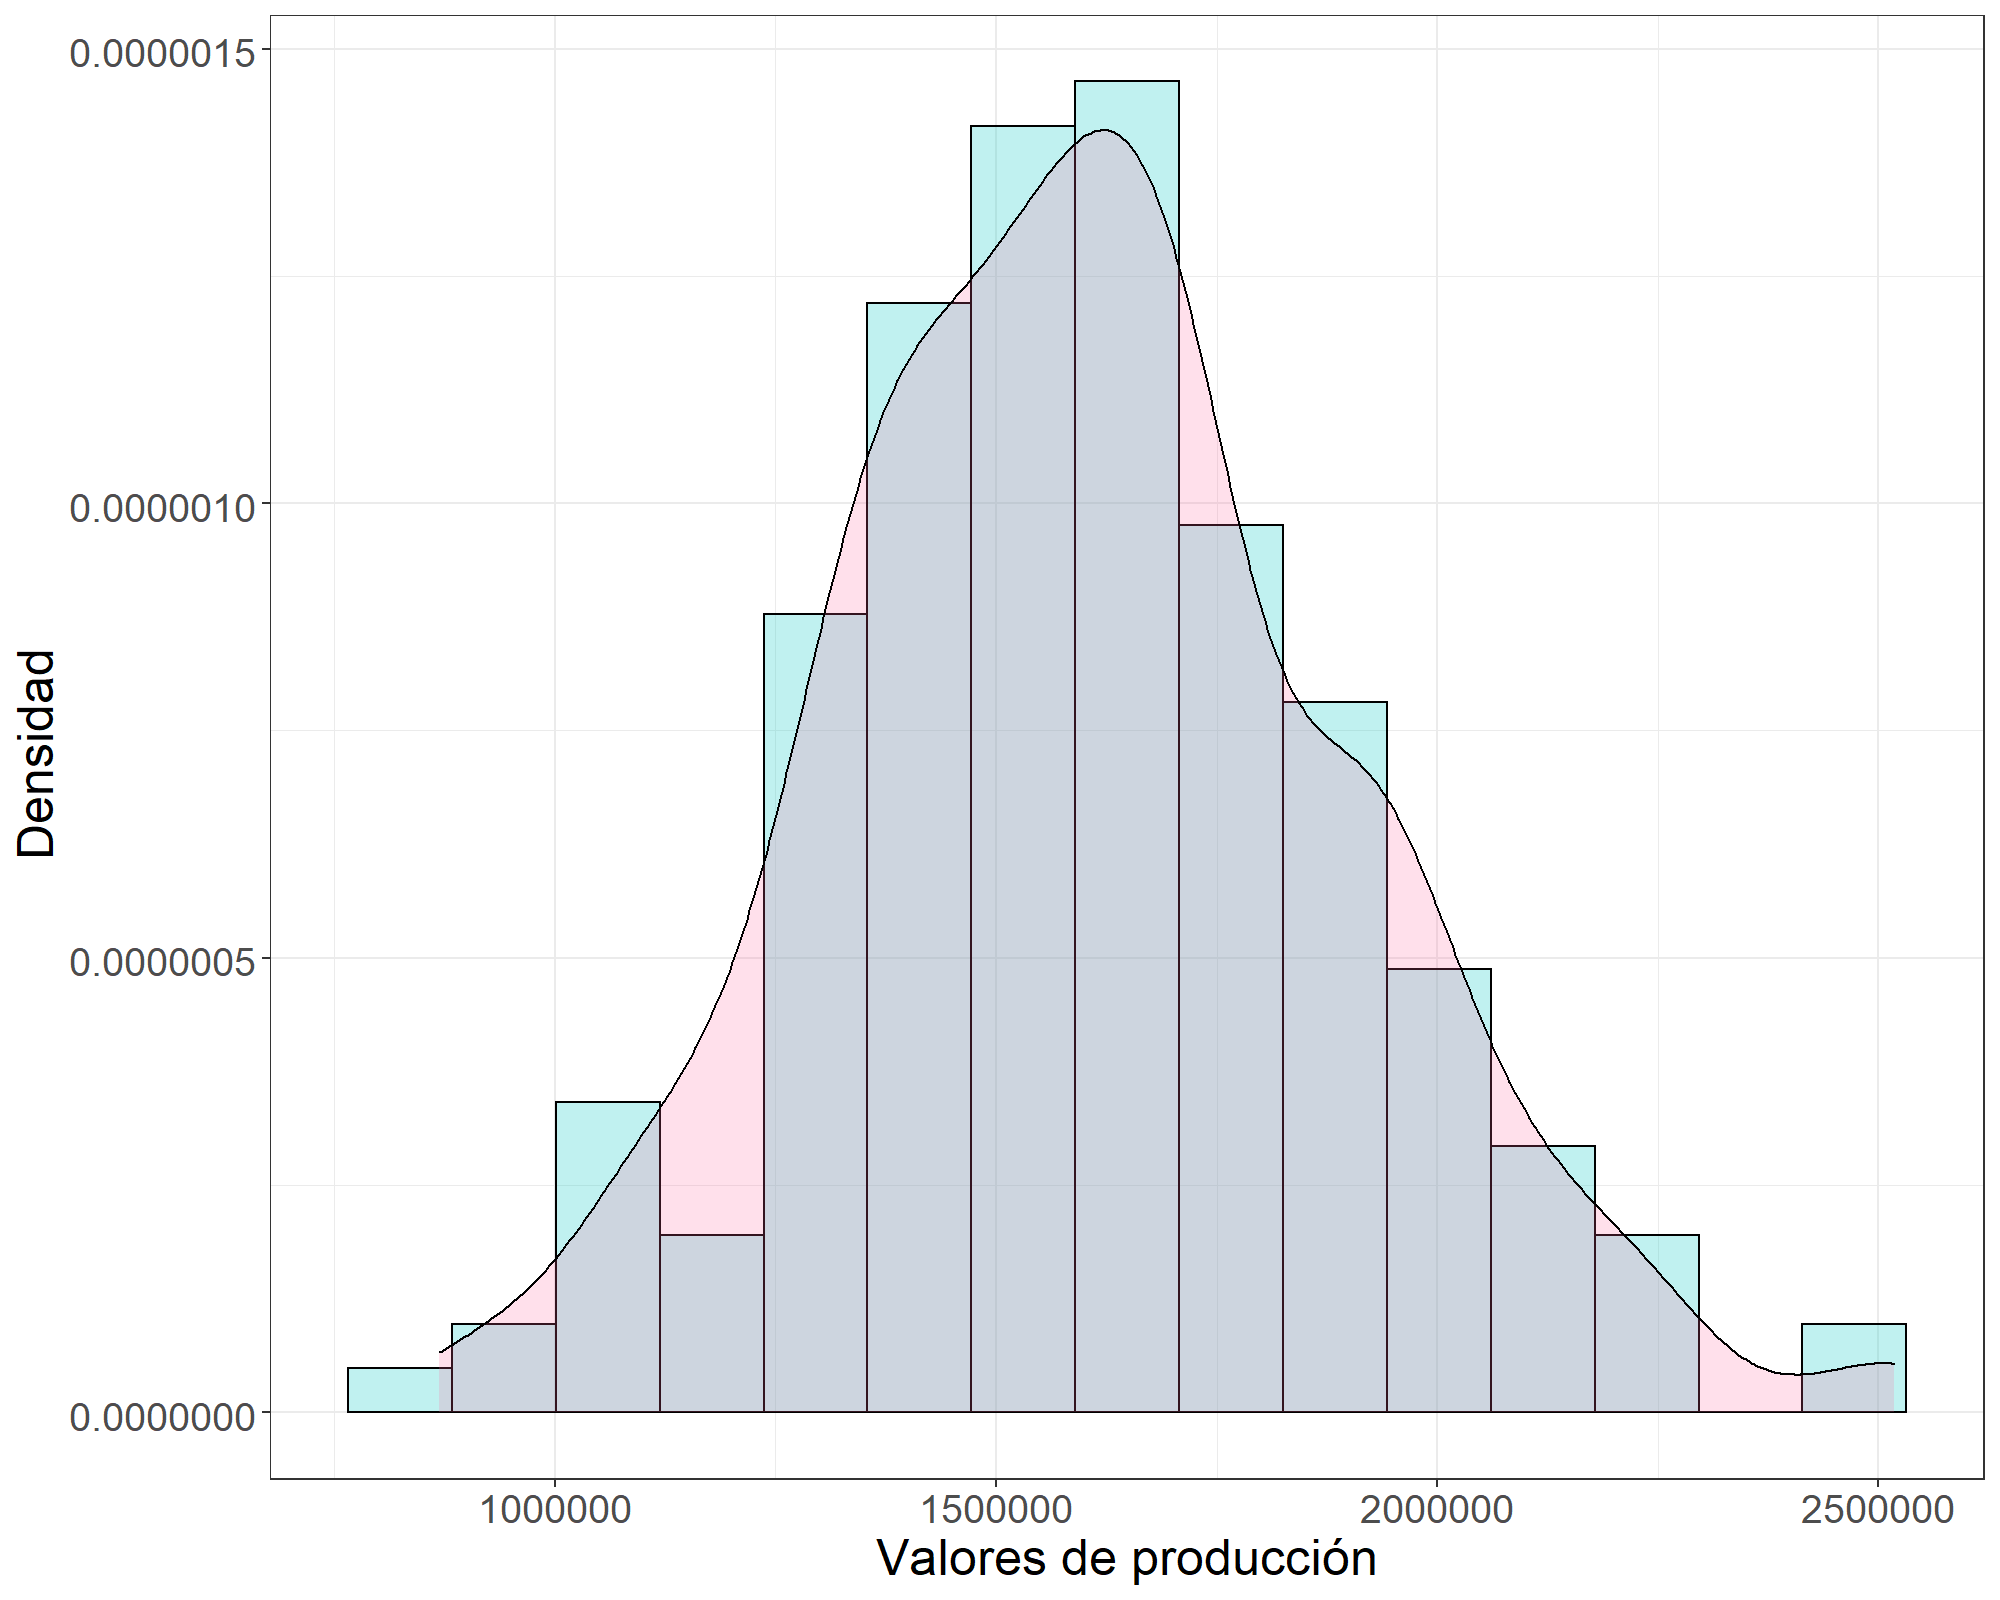
\includegraphics[scale=0.32]{figuras/ShapiroAgua.png}}
\label{fig:a}
\centering
\subfigure[Petróleo y petroquímica]{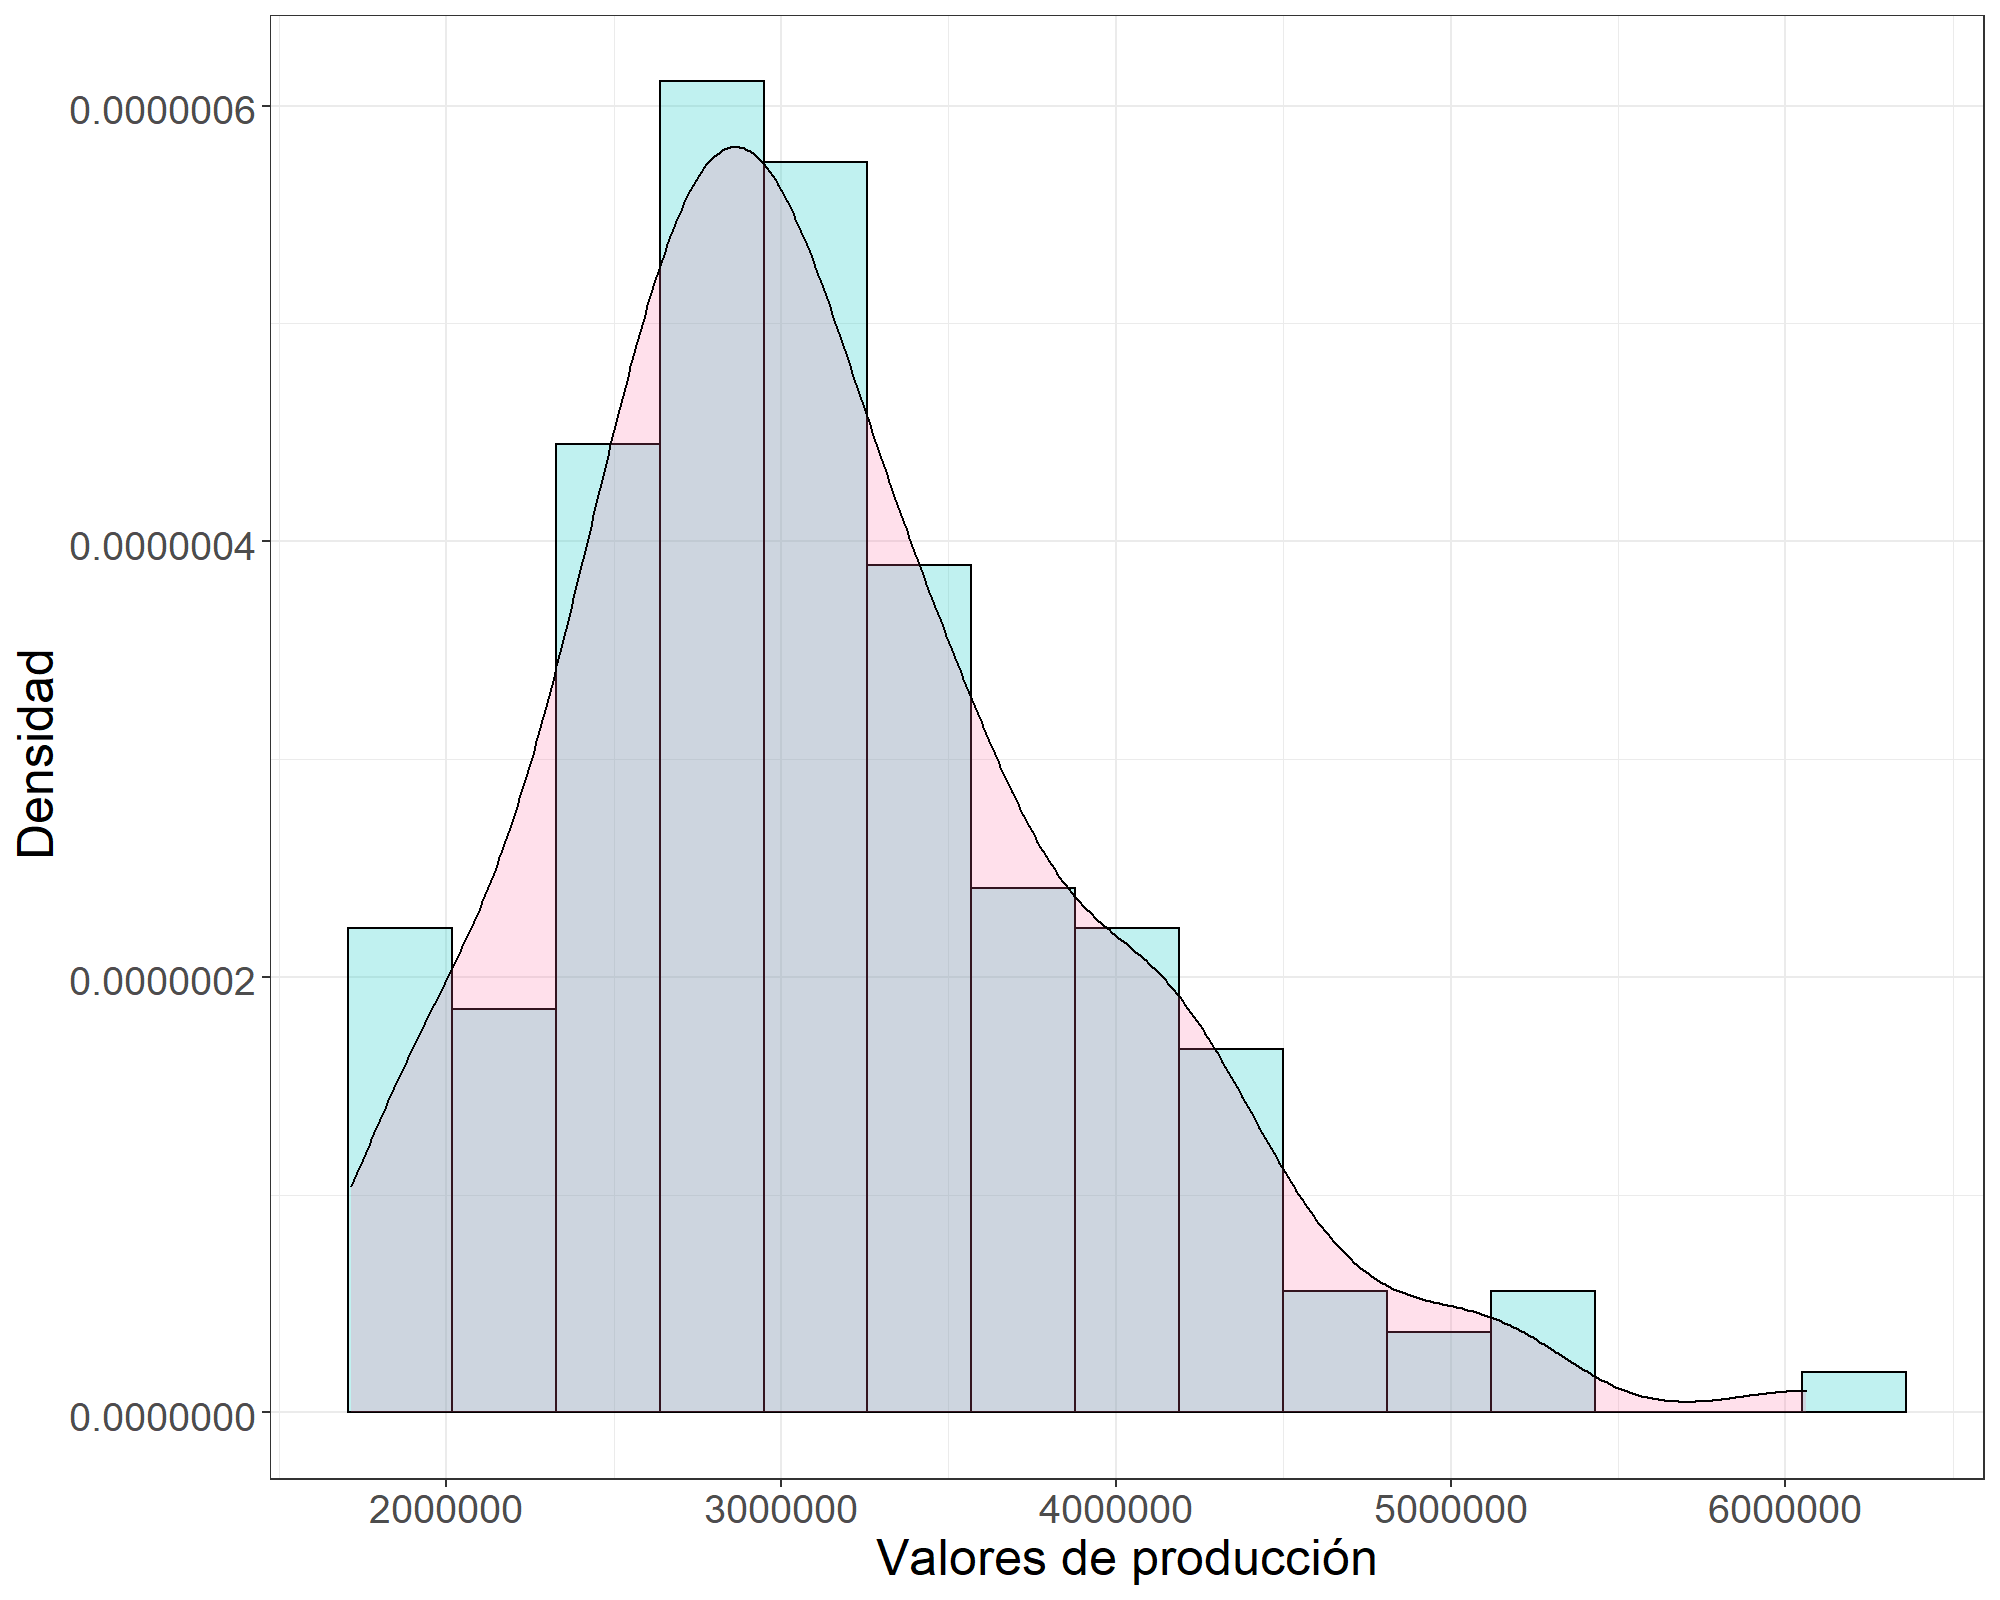
\includegraphics[scale=0.32]{figuras/ShapiroPetro.png}}
\label{fig:b}
\centering
\subfigure[Otras construcciones]{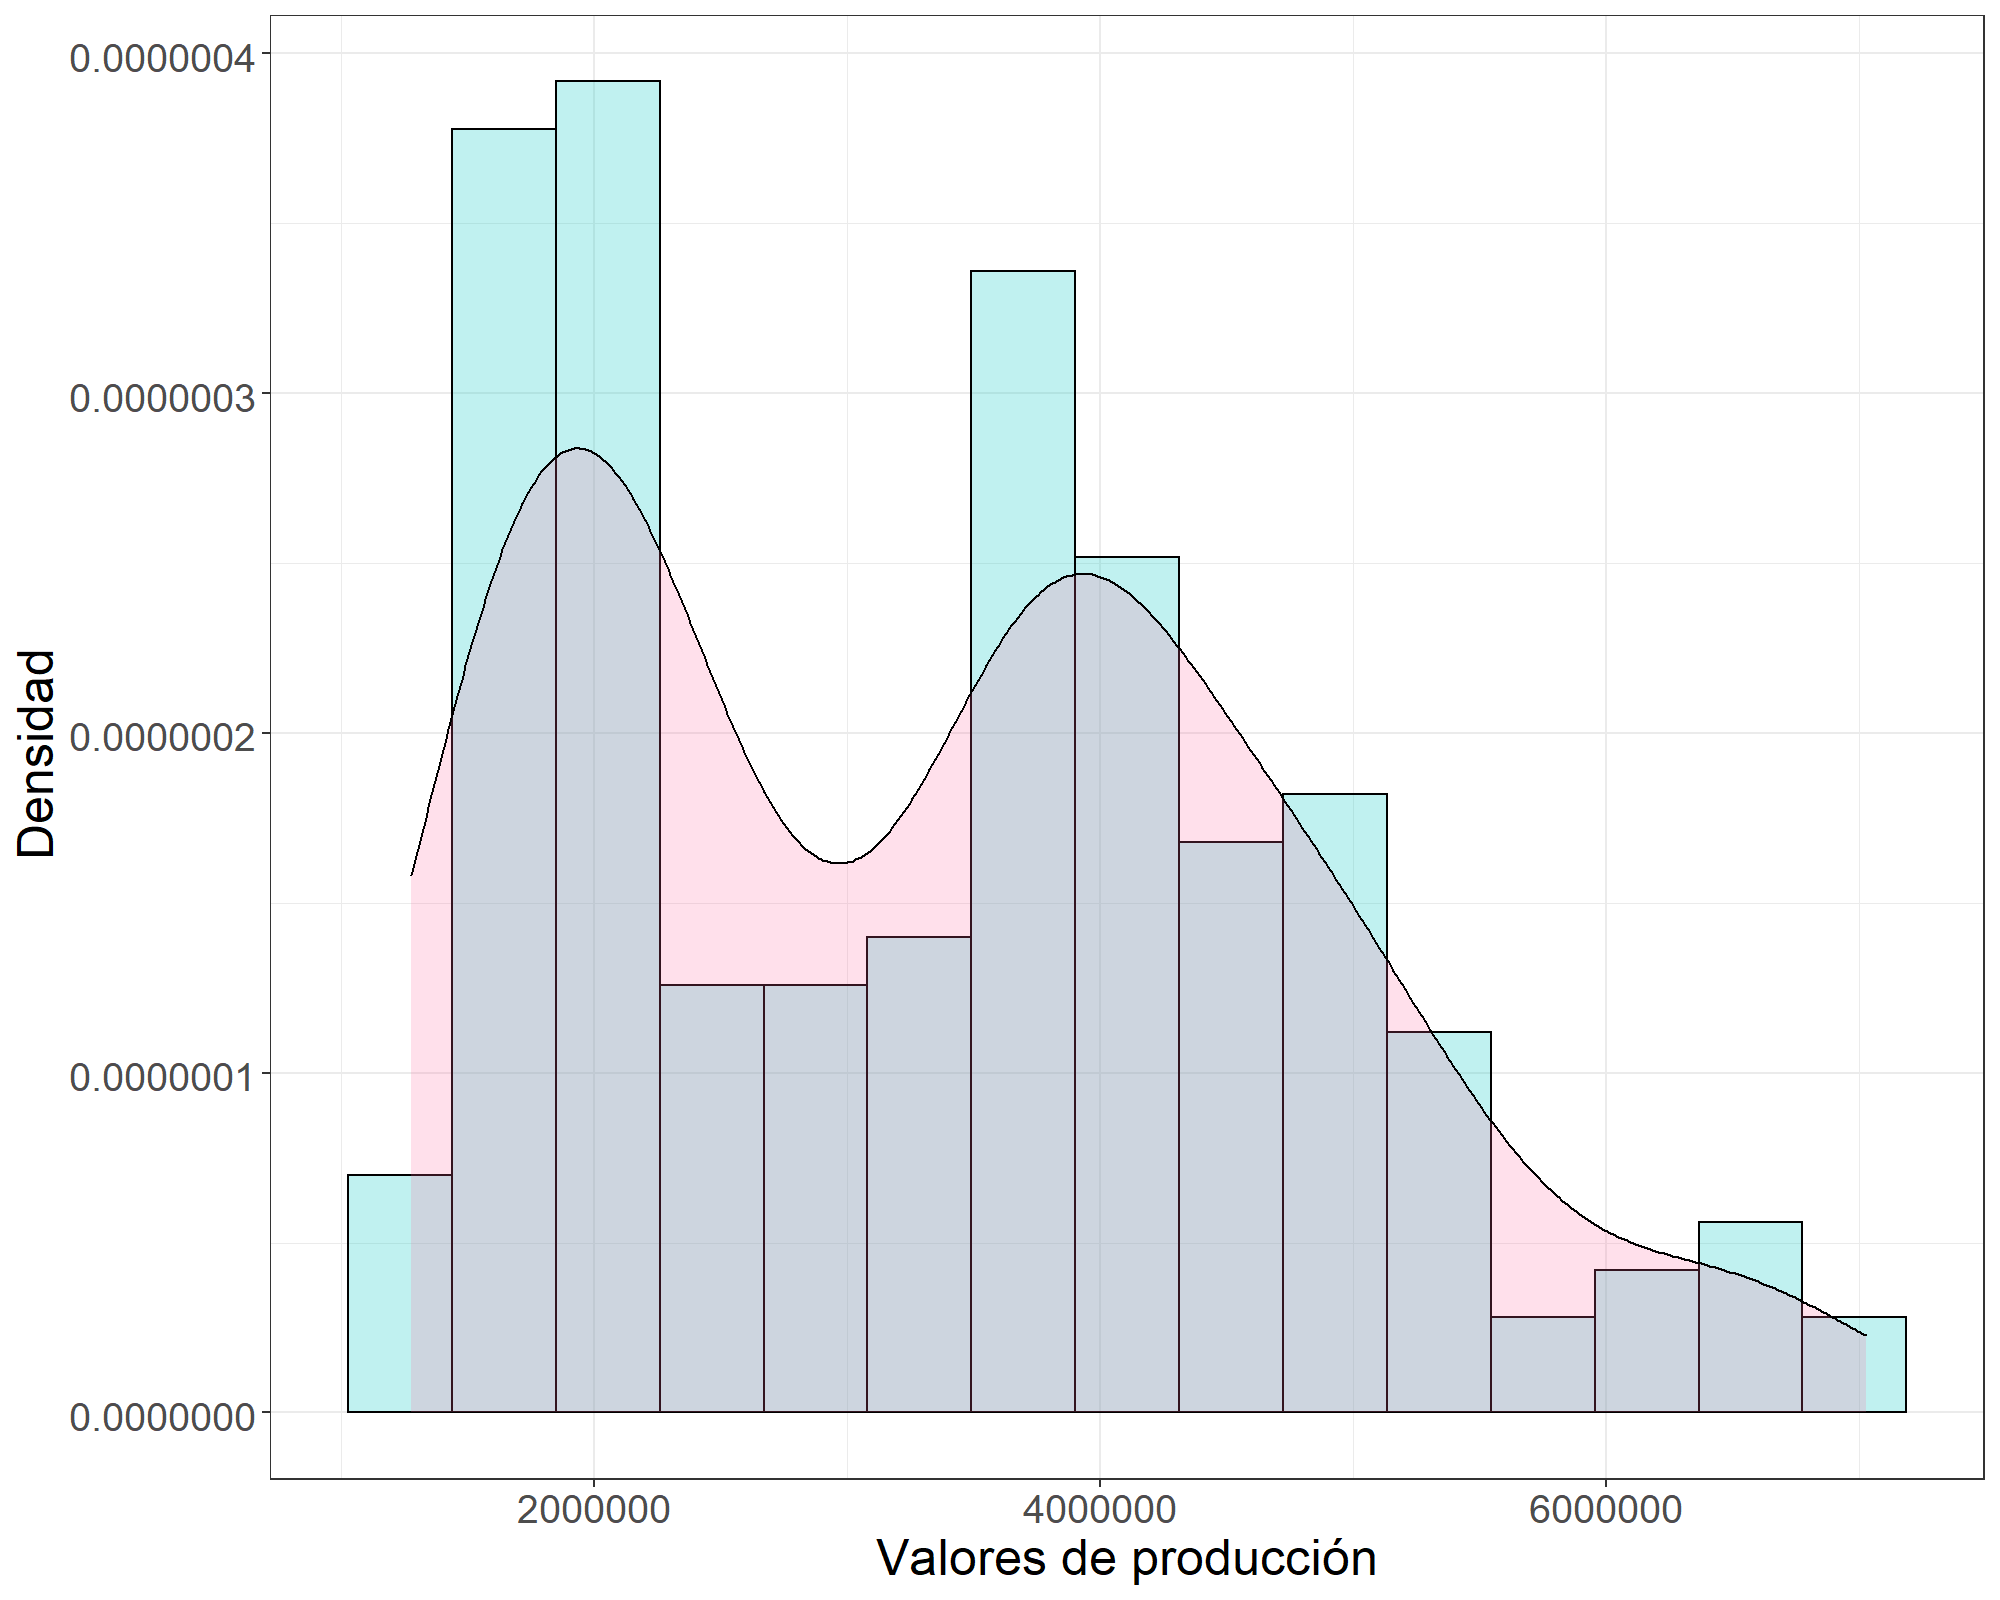
\includegraphics[scale=0.32]{figuras/ShapiroOtras.png}}
\label{fig:c}
\vspace{-0.2cm}
\caption{Histogramas de distribución de los datos por tipo de obras}
\label{fig:4} 
\end{figure}

\subsection{Prueba t de una muestra}
\label{sec:10}
la prueba t de una muestra, es una prueba paramétrica, se utiliza para probar si la media de una muestra puede ser un valor especifico. Al ser paramétrica como premisa necesita que la muestra siga una distribución normal. De los resultados en el cuadro \ref{tab:6} de la página \pageref{tab:6}, podemos concluir que solo podemos aplicar la prueba t a los datos del tipo de obras Agua, riego y saneamiento, por ser los únicos que siguen una distribución normal.

La prueba se realiza con un $\alpha$ = 0.05, y la hipótesis planteada es la siguiente: 
\begin{equation}\label{eq:1}
H_{0}:\text{La}\:  \mu\:  \text{de los de los valores de producción es 1600000},    
\end{equation}
\begin{equation}\label{eq:2}
 H_{1}:\text{La}\: \mu \: \text{de los de los valores de producción diferente 1600000}. 
\end{equation}
Los resultados obtenidos en la prueba, con un estadístico \textbf{t} = 0.3014 y un \textbf{valor p} = 0.7635 mayor que $\alpha$, se puede concluir que no hay evidencias para rechazar la hipótesis $H_{0}$, por lo tanto la media de los valores de producción es 1600000 con un intervalo de confianza de 95\%. Esto se puede observar en la figura \ref{fig:7} de la página \pageref{fig:7}.



\begin{figure}
\centering
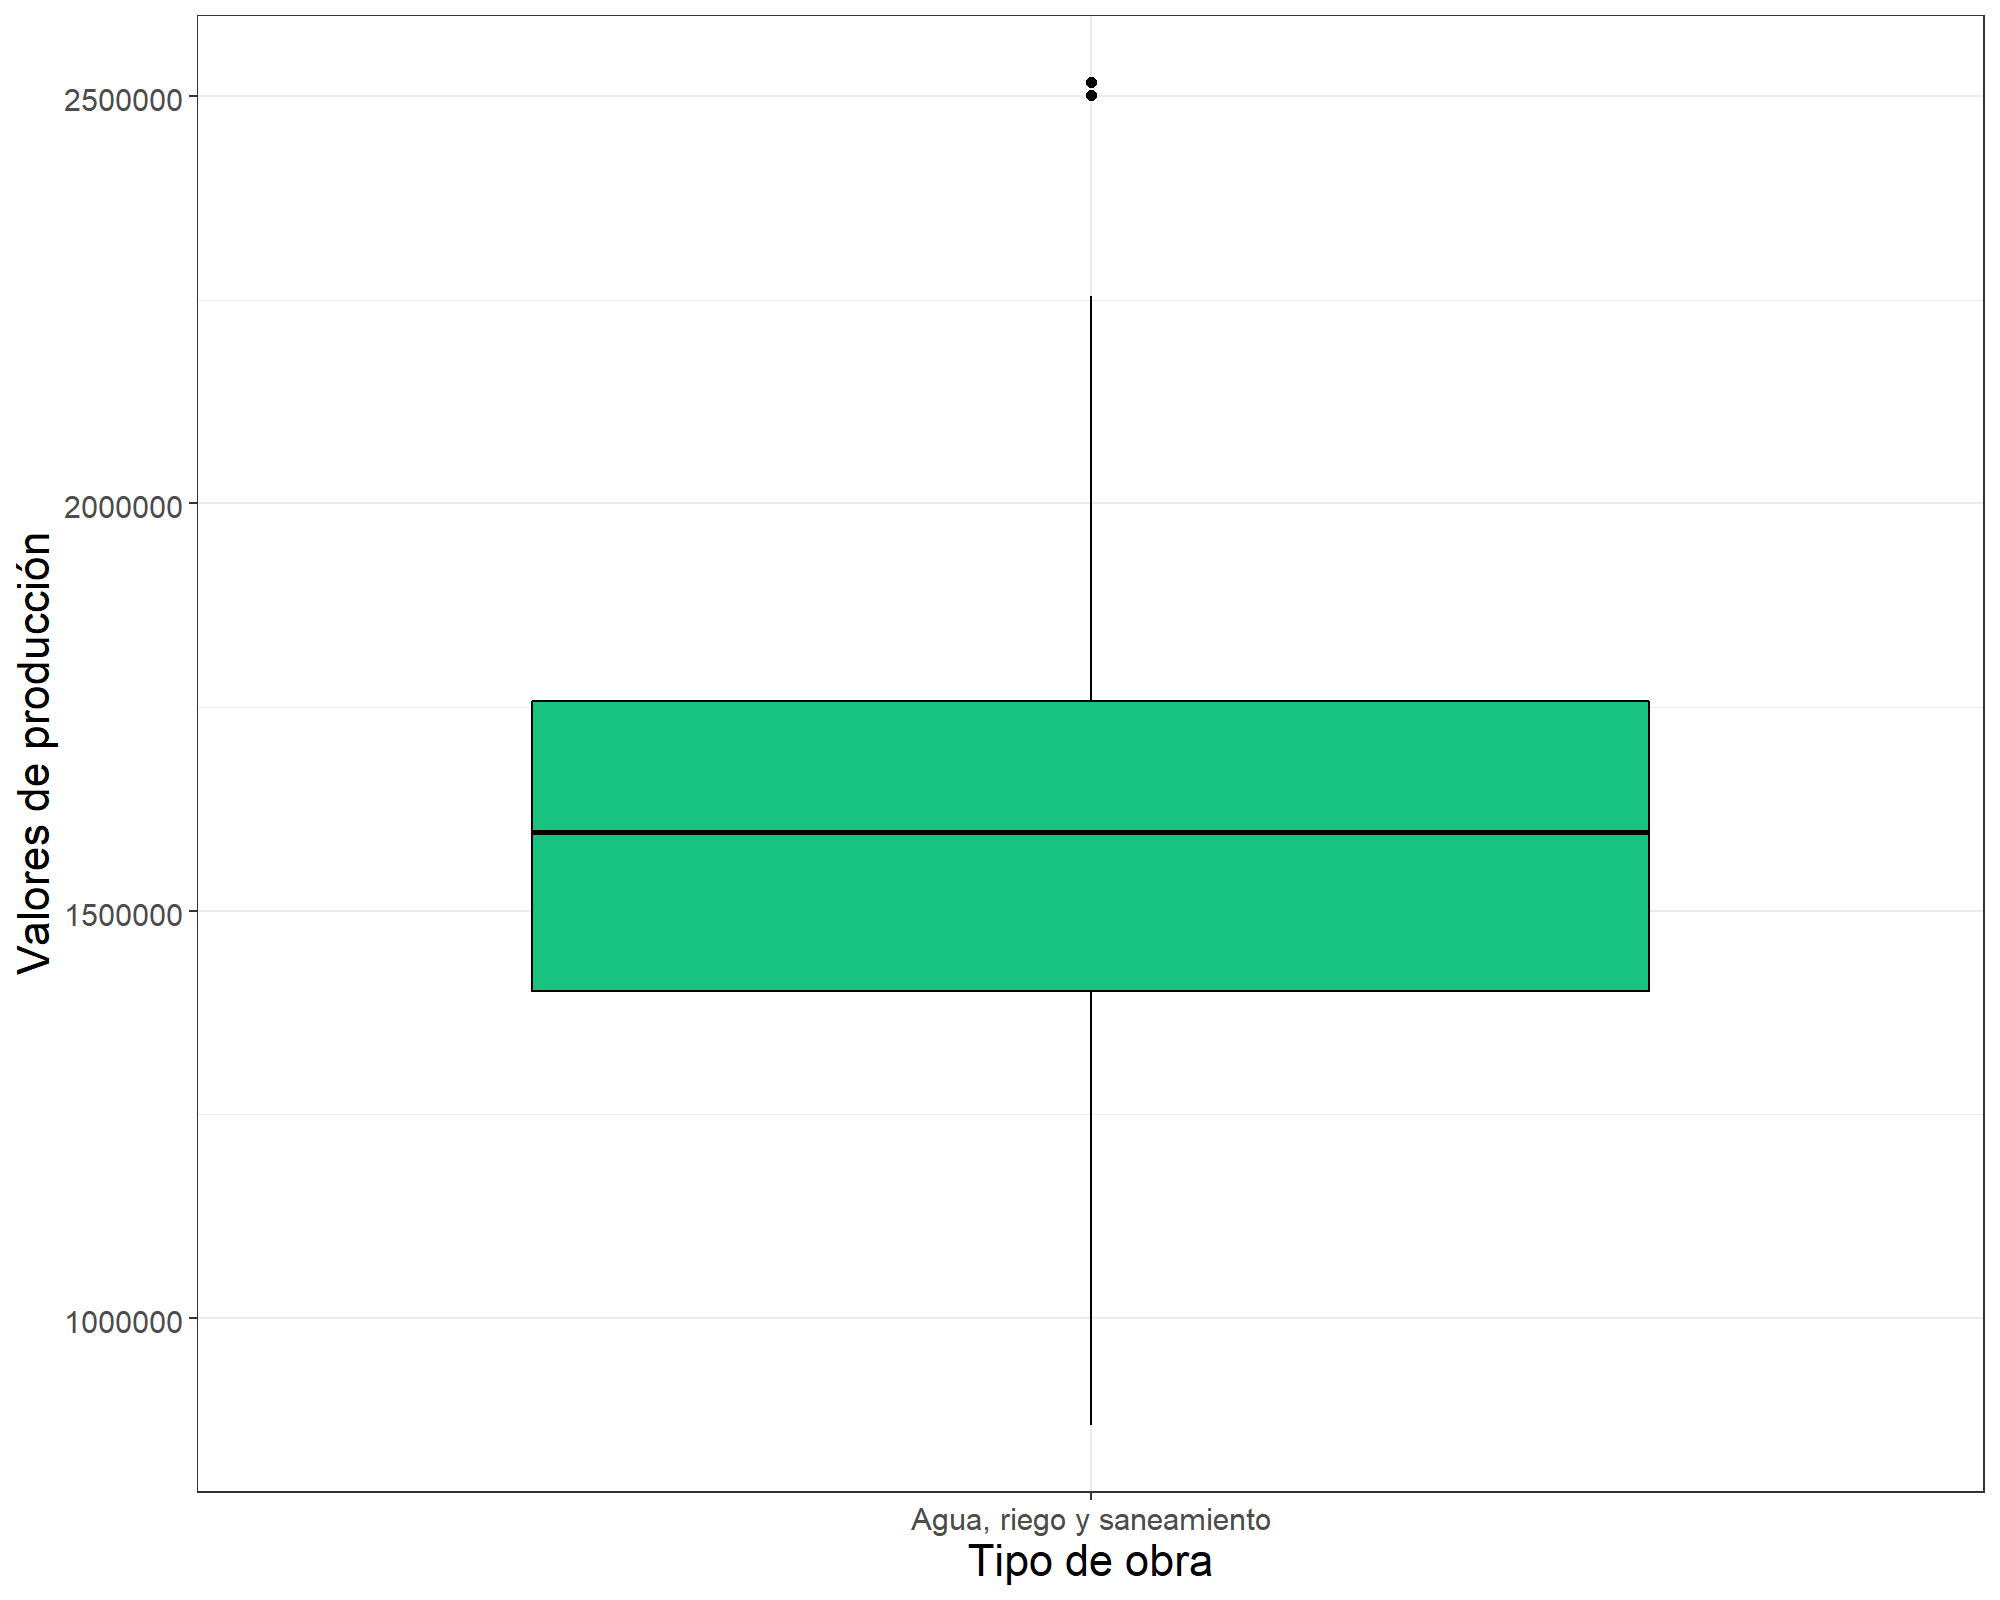
\includegraphics[scale=0.45]{figuras/TestT.png}
\caption{Diagrama de caja y bigotes del tipo de obra Agua, riego y saneamiento}
\label{fig:7}
\end{figure}

\subsection{Prueba de rango con signo de Wilcoxon}
La prueba de rango con signo de Wilcoxon puede verse como una alternativa a la prueba t, dado que su objetivo es determinar si la media de una muestra es un valor especifico sin tener en cuenta el supuesto que la muestra sigue una distribución normal.

Para la prueba se utilizan los datos pertenecientes al tipo de obra Petróleo y petroquímica, debido a que estos no siguen una distribución normal. La prueba se realiza con un $\alpha$ = 0.05, y la hipótesis planteada es la siguiente: 
\begin{equation}\label{eq:1}
H_{0}:\text{La}\:  \mu\:  \text{de los de los valores de producción es 300000},    
\end{equation}
\begin{equation}\label{eq:2}
 H_{1}:\text{La}\: \mu \: \text{de los de los valores de producción diferente 3000000}. 
\end{equation}
Los resultados obtenidos en la prueba, con un estadístico \textbf{V} = 8399 y un \textbf{valor p} = 0.2375 mayor que $\alpha$, se puede concluir que no hay evidencias para rechazar la hipótesis $H_{0}$, por lo tanto la media de los valores de producción de las obras Petróleo y petroquímica es 3000000 con un intervalo de confianza de 95\%. Esto se puede observar en la figura \ref{fig:8} de la página \pageref{fig:8}.

\begin{figure}
\centering
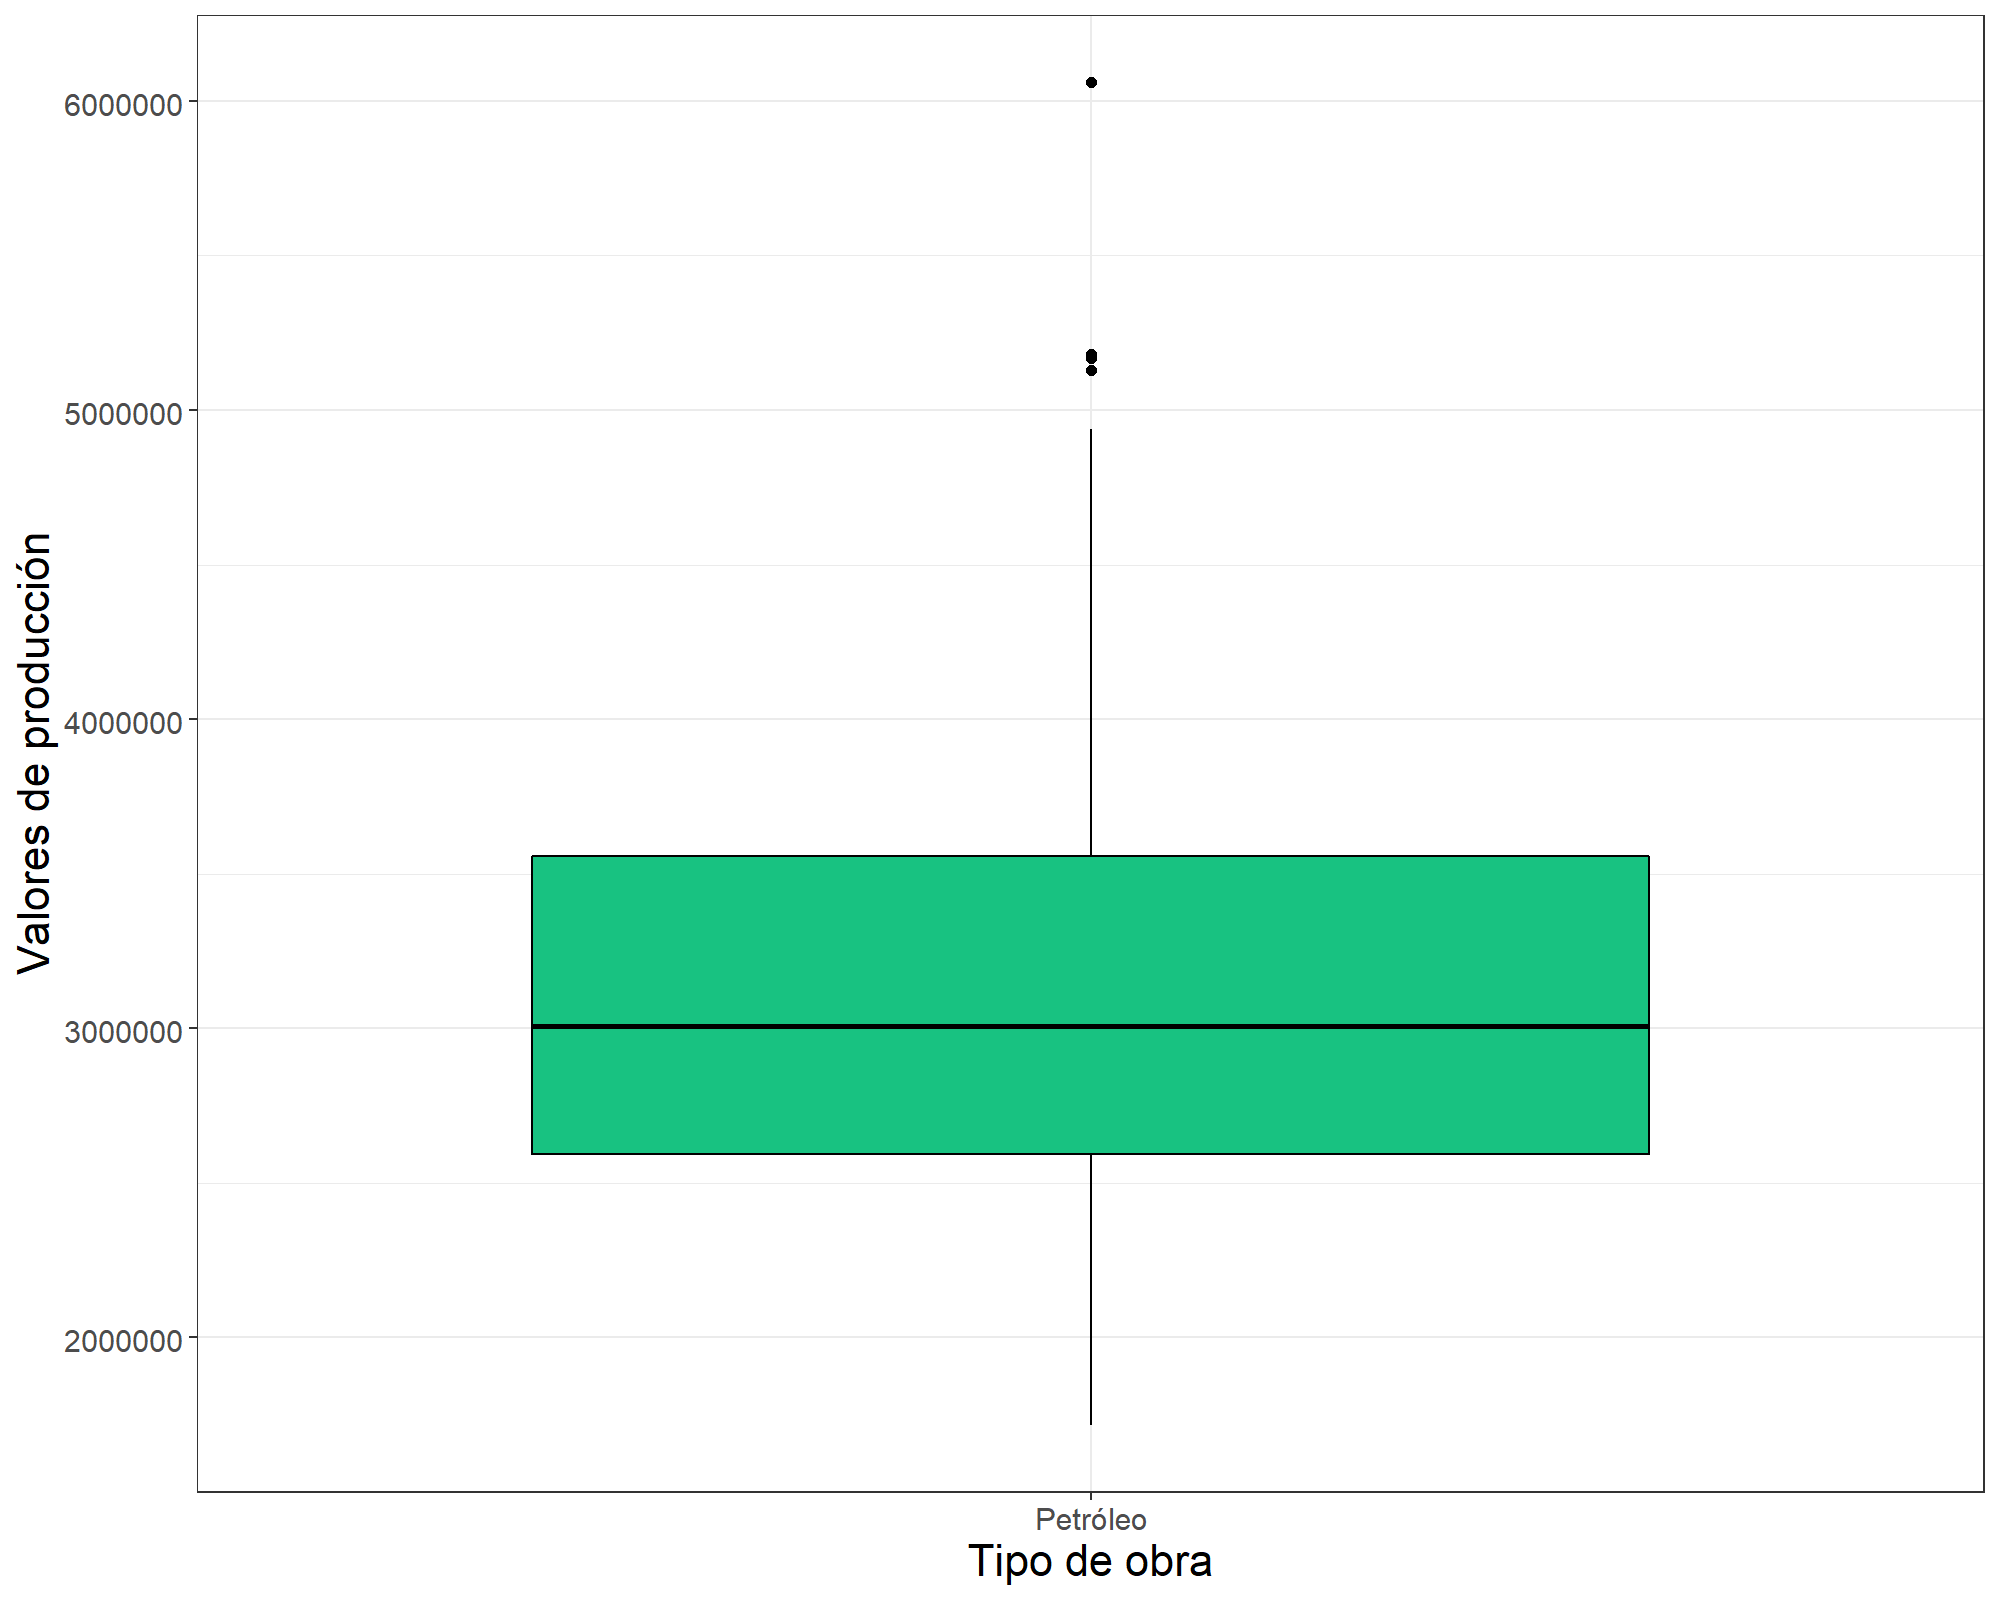
\includegraphics[scale=0.45]{figuras/Wil.png}
\caption{Diagrama de caja y bigotes del tipo de obra Petróleo y petroquímica}
\label{fig:8}
\end{figure}

\subsection{Prueba t de dos muestras de rangos de Wilcoxon}
La Prueba t de dos muestras de rangos de Wilcoxon tiene como objetivo comparar las medias de dos muestras que no siguen una distribución normal. 

Para esta prueba se utilizan los datos pertenecientes al tipo de obra Petróleo y petroquímica y Otras construcciones, debido a que estos no siguen una distribución normal. La prueba se realiza con un $\alpha$ = 0.05, y la hipótesis planteada es la siguiente: 
\begin{equation}\label{eq:1}
H_{0}:\mu\:\text{(Petróleo y petroquímica)} = \mu\:\text{(Otras construcciones)},    
\end{equation}
\begin{equation}\label{eq:2}
 H_{1}:\mu\:\text{(Petróleo y petroquímica)} \neq \mu\:\text{(Otras construcciones)}. 
\end{equation}
Los resultados obtenidos en la prueba, con un estadístico \textbf{W} = 14364 y un \textbf{valor p} = 0.7954 mayor que $\alpha$, se puede concluir que no hay evidencias para rechazar la hipótesis $H_{0}$, por lo tanto la media de los valores de producción de las obras Petróleo y Otras construcciones tienen la misma media con un intervalo de confianza de 95\%. Esto se puede observar en la figura \ref{fig:9} de la página \pageref{fig:9}.

\begin{figure}
\centering
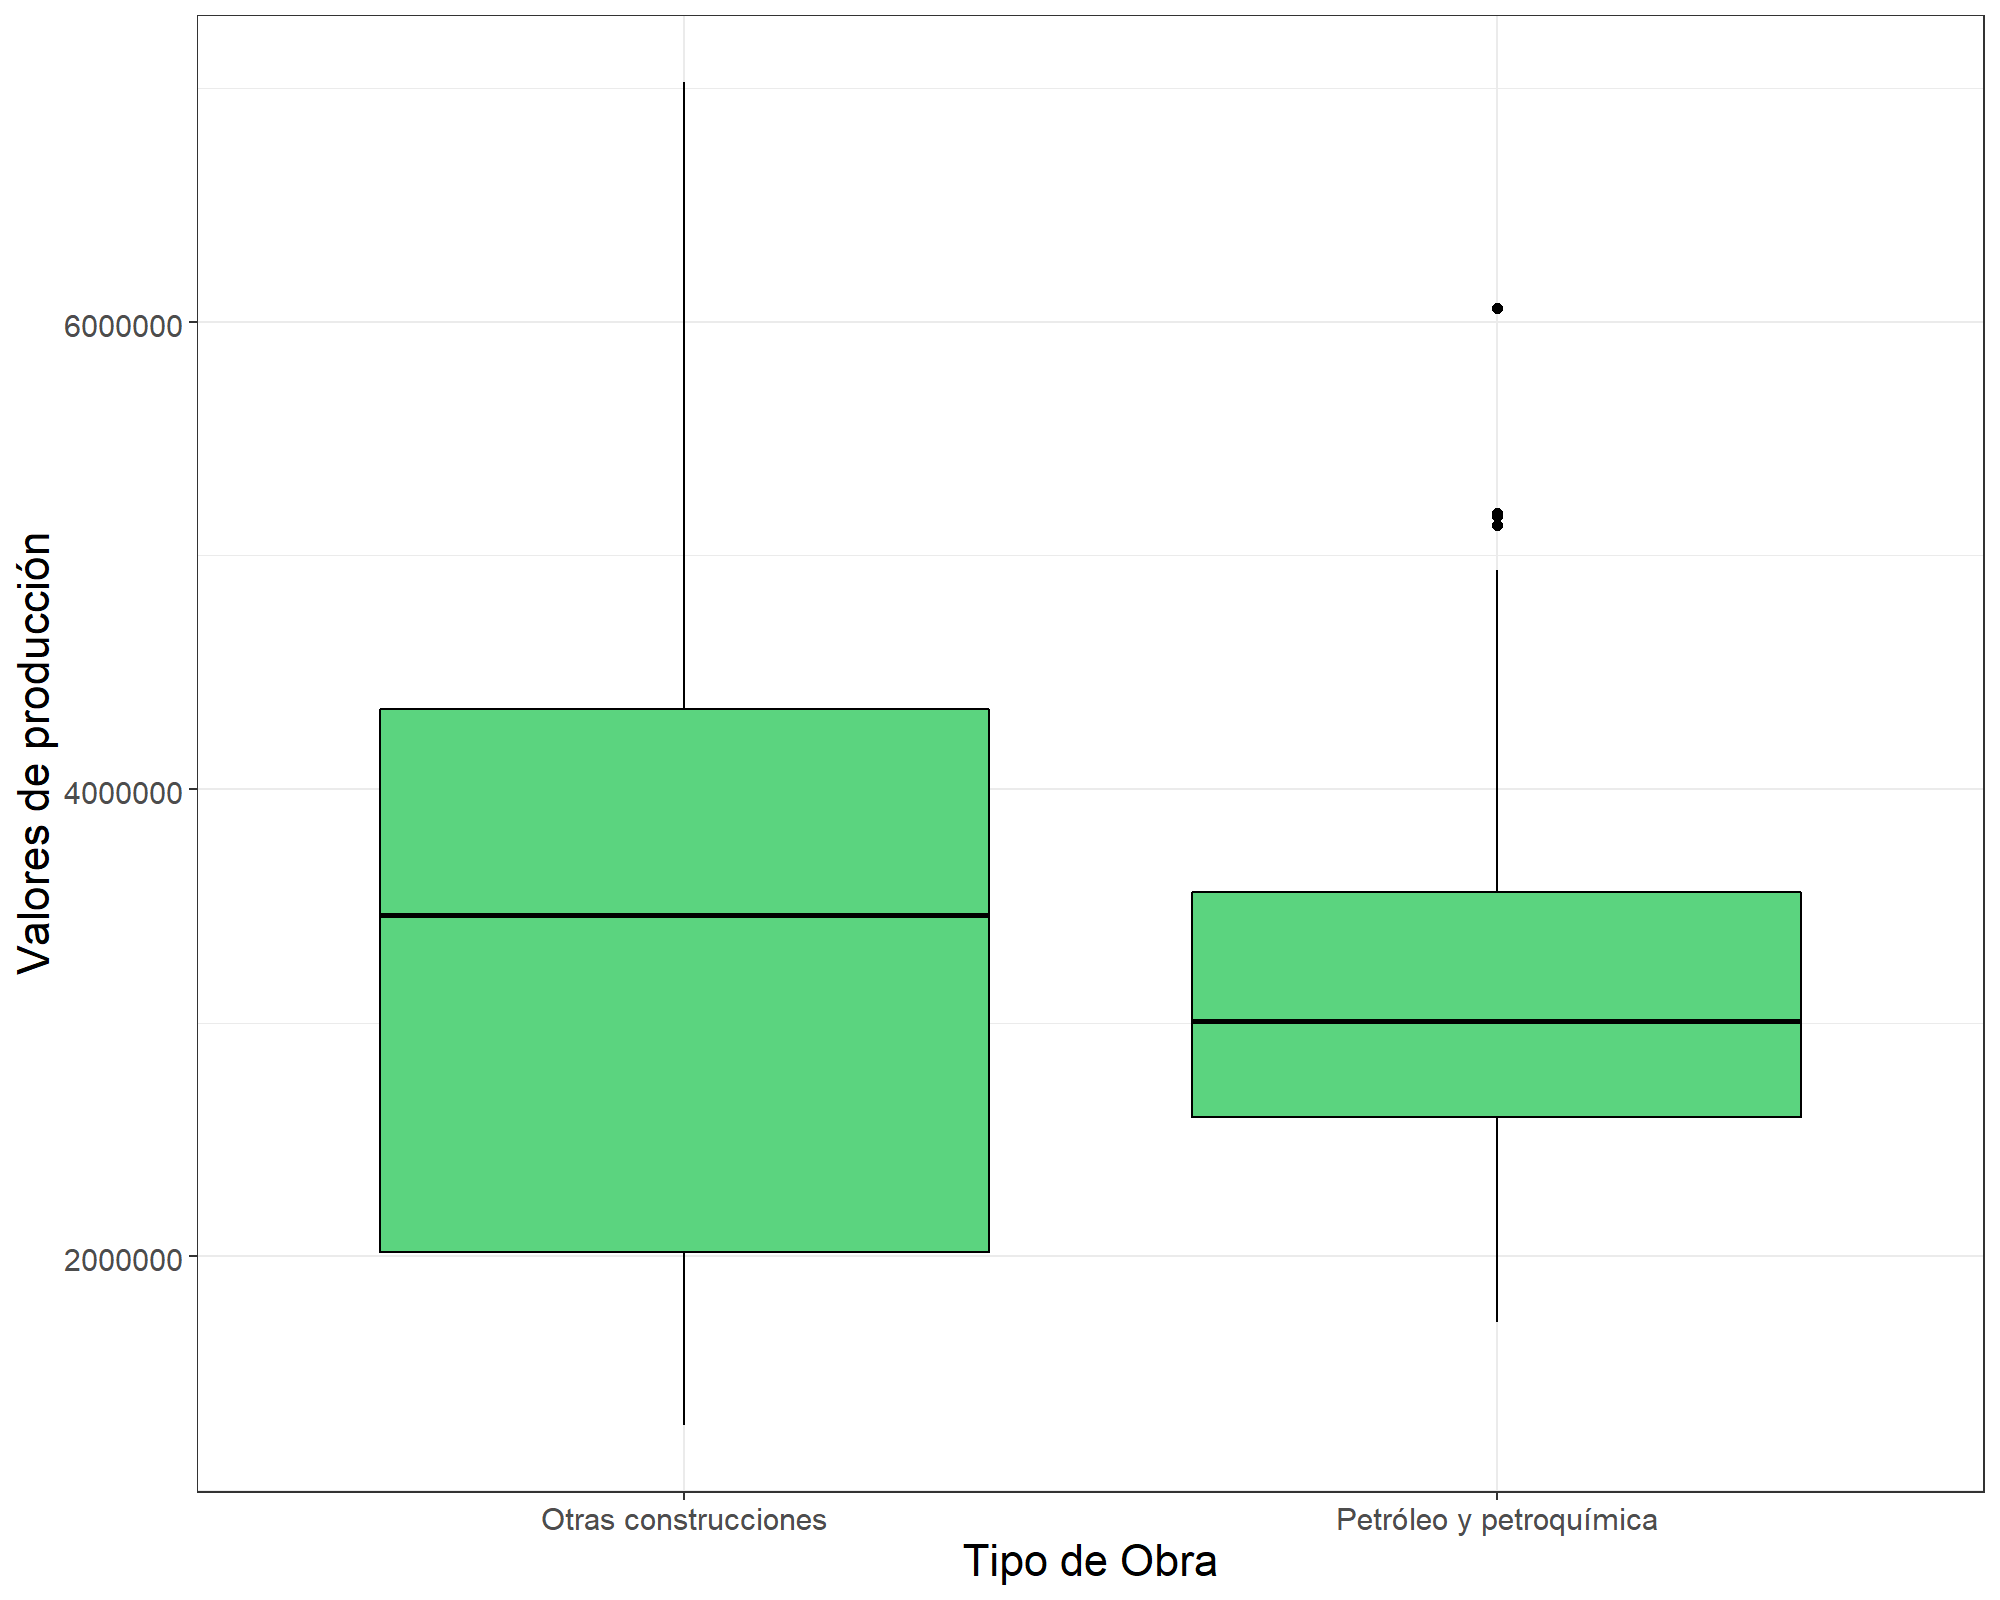
\includegraphics[scale=0.50]{figuras/WilDoble.png}
\caption{Diagrama de caja y bigotes del tipo de obra Petróleo y petroquímica y Otras construcciones}
\label{fig:9}
\end{figure}

\subsection{Prueba de Kolmogorov y Smirnov}
La prueba de Kolmogorov-Smirnov se utiliza para comprobar si dos muestras siguen la misma distribución.

Para esta prueba se utilizan los datos pertenecientes al tipo de obra Agua, riego y saneamiento y datos creados con la función \textit{rnorm} de R. Con el objetivo de verificar los resultados de la prueba Shapiro-Wilk realizada en la \ref{sec:10}. La prueba se realiza con un $\alpha$ = 0.05, y la hipótesis planteada es la siguiente:
\begin{equation}\label{eq:1}
H_{0}:\text{(la distribución de Agua, riego y saneamiento)} = \text{(la distribución \textit{rnorm})}, 
\end{equation}
\begin{equation}\label{eq:2}
H_{1}: \text{(la distribución de Agua, riego y saneamiento)} \neq \text{(la distribución \textit{rnorm})}. 
\end{equation}
Los resultados obtenidos en la prueba, con una distancia de Kolmogorov-Smirnov \textbf{D} = 0.086207 y un \textbf{valor p} = 0.5375 mayor que $\alpha$, se puede concluir que no hay evidencias para rechazar la hipótesis $H_{0}$, por lo tanto los valores de producción de  tipo de obra Agua, riego y saneamiento siguen una distribución normal con un intervalo de confianza de 95\%. Esto se puede observar en la figura \ref{fig:10} de la página \pageref{fig:10}.

\begin{figure}
\centering
\subfigure[Diagrama de densidad de Agua, riego y saneamiento superpuesto al simulado con \textit{rnorm}]{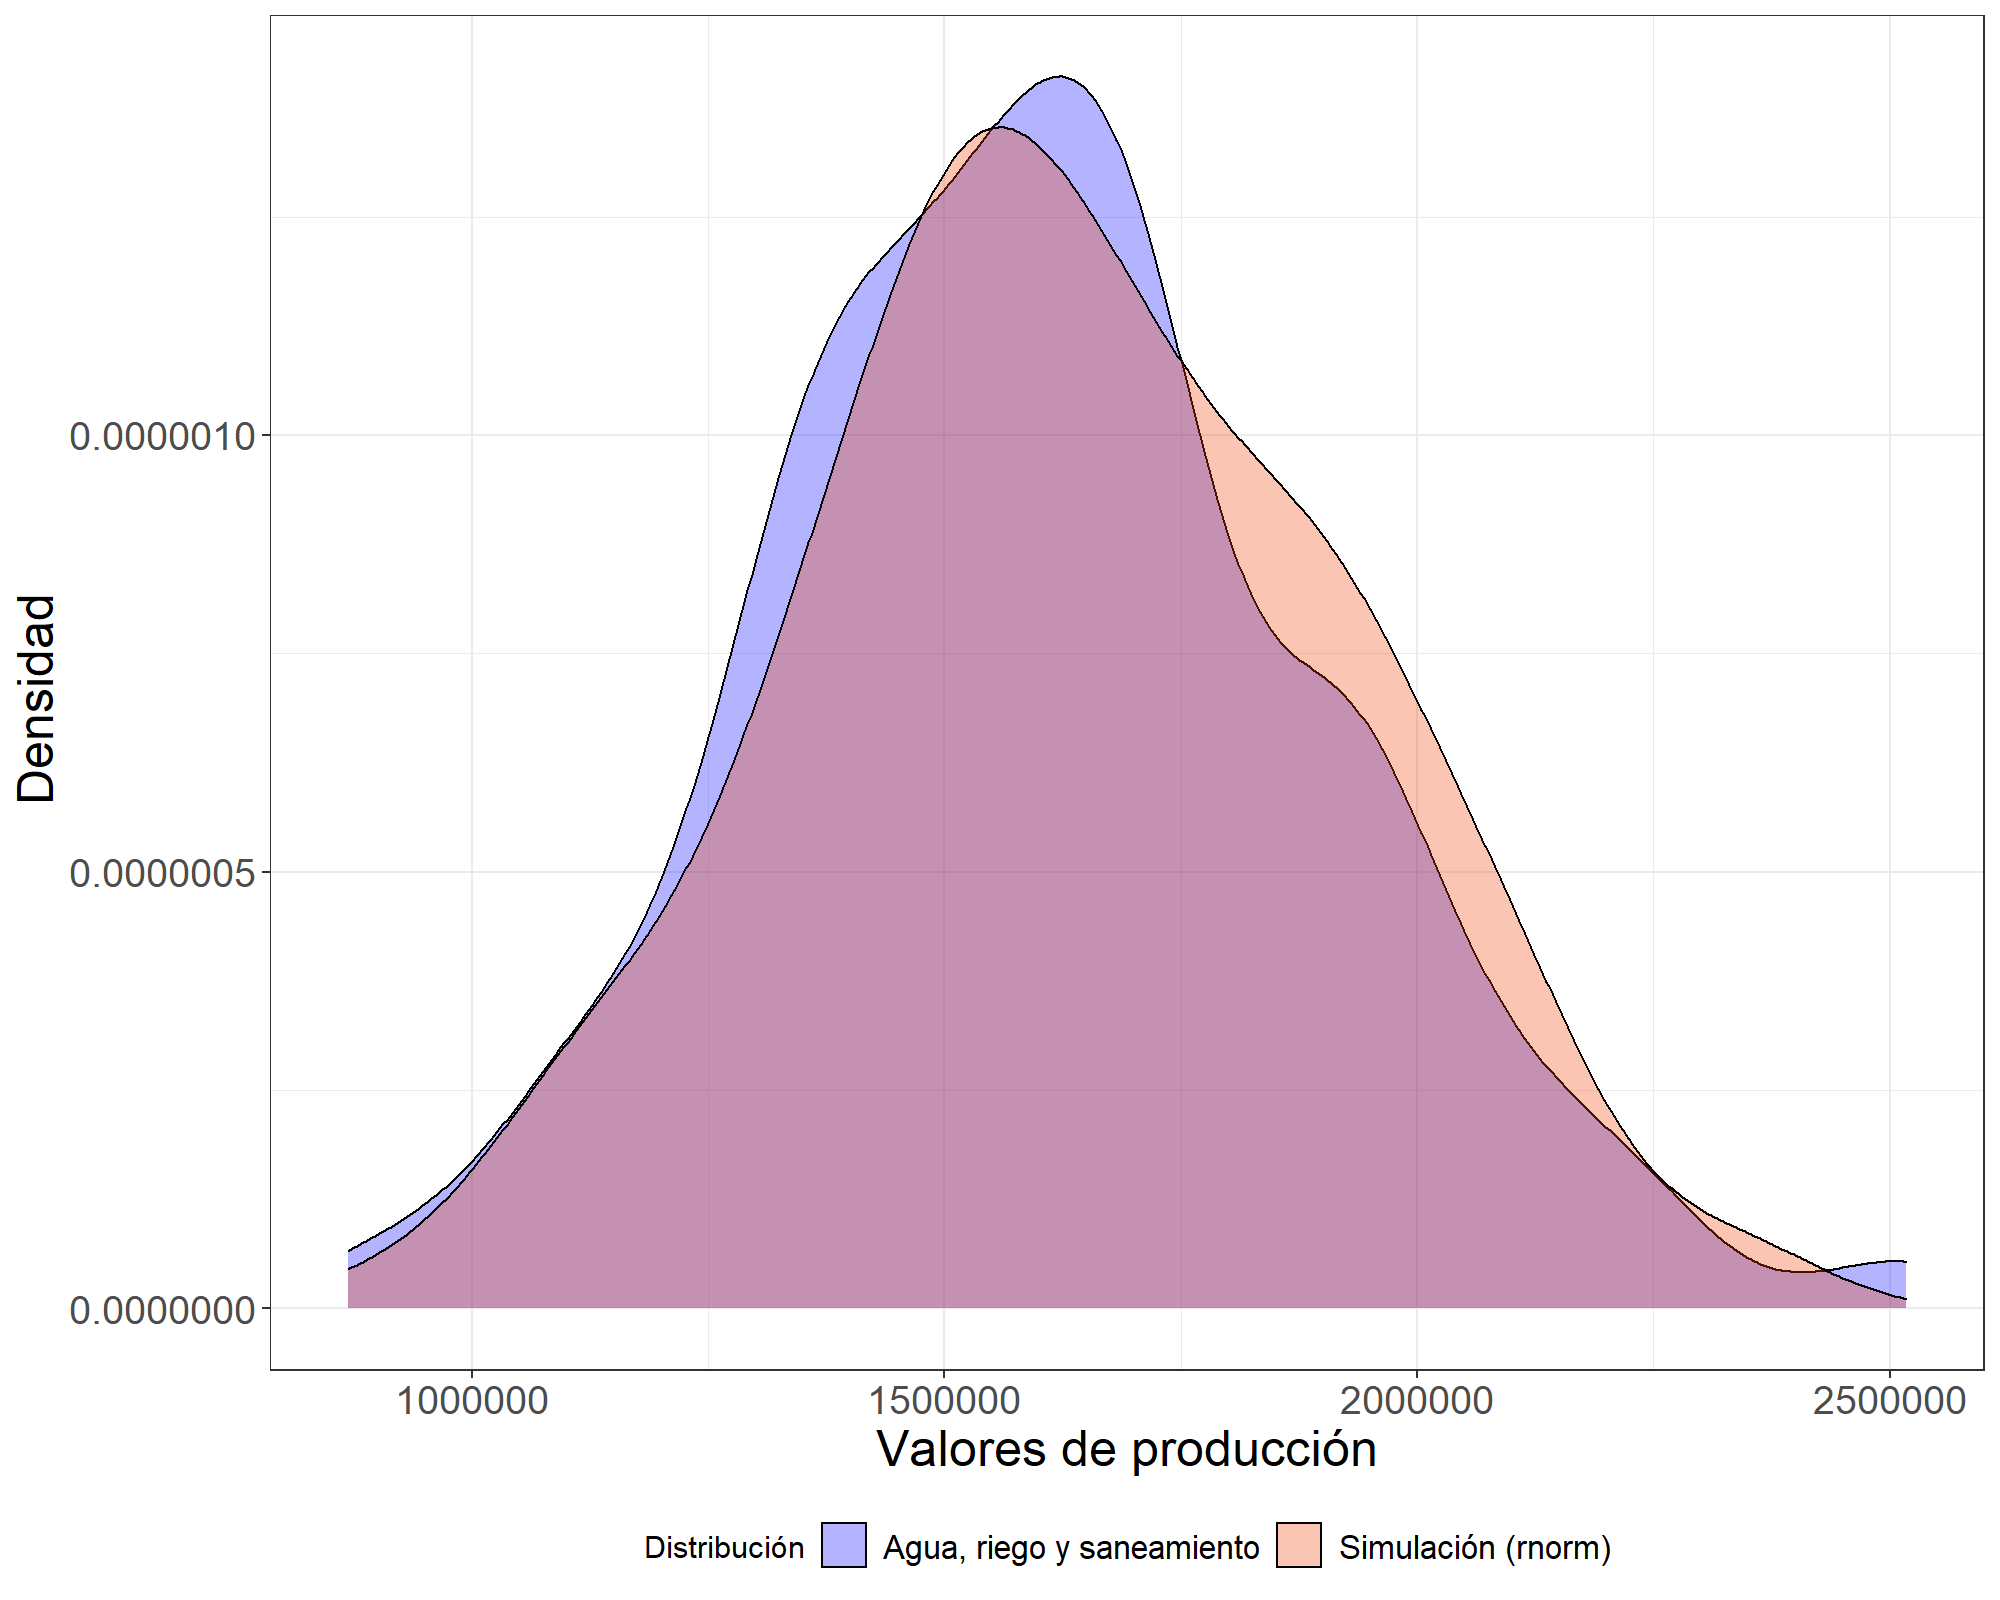
\includegraphics[scale=0.47]{figuras/Dens1.png}}
\label{fig:e}
\centering
\subfigure[[Diferencia de Kolmogorov-Smirnov entre Agua, riego y saneamiento superpuesto y la  simulación con \textit{rnorm}]{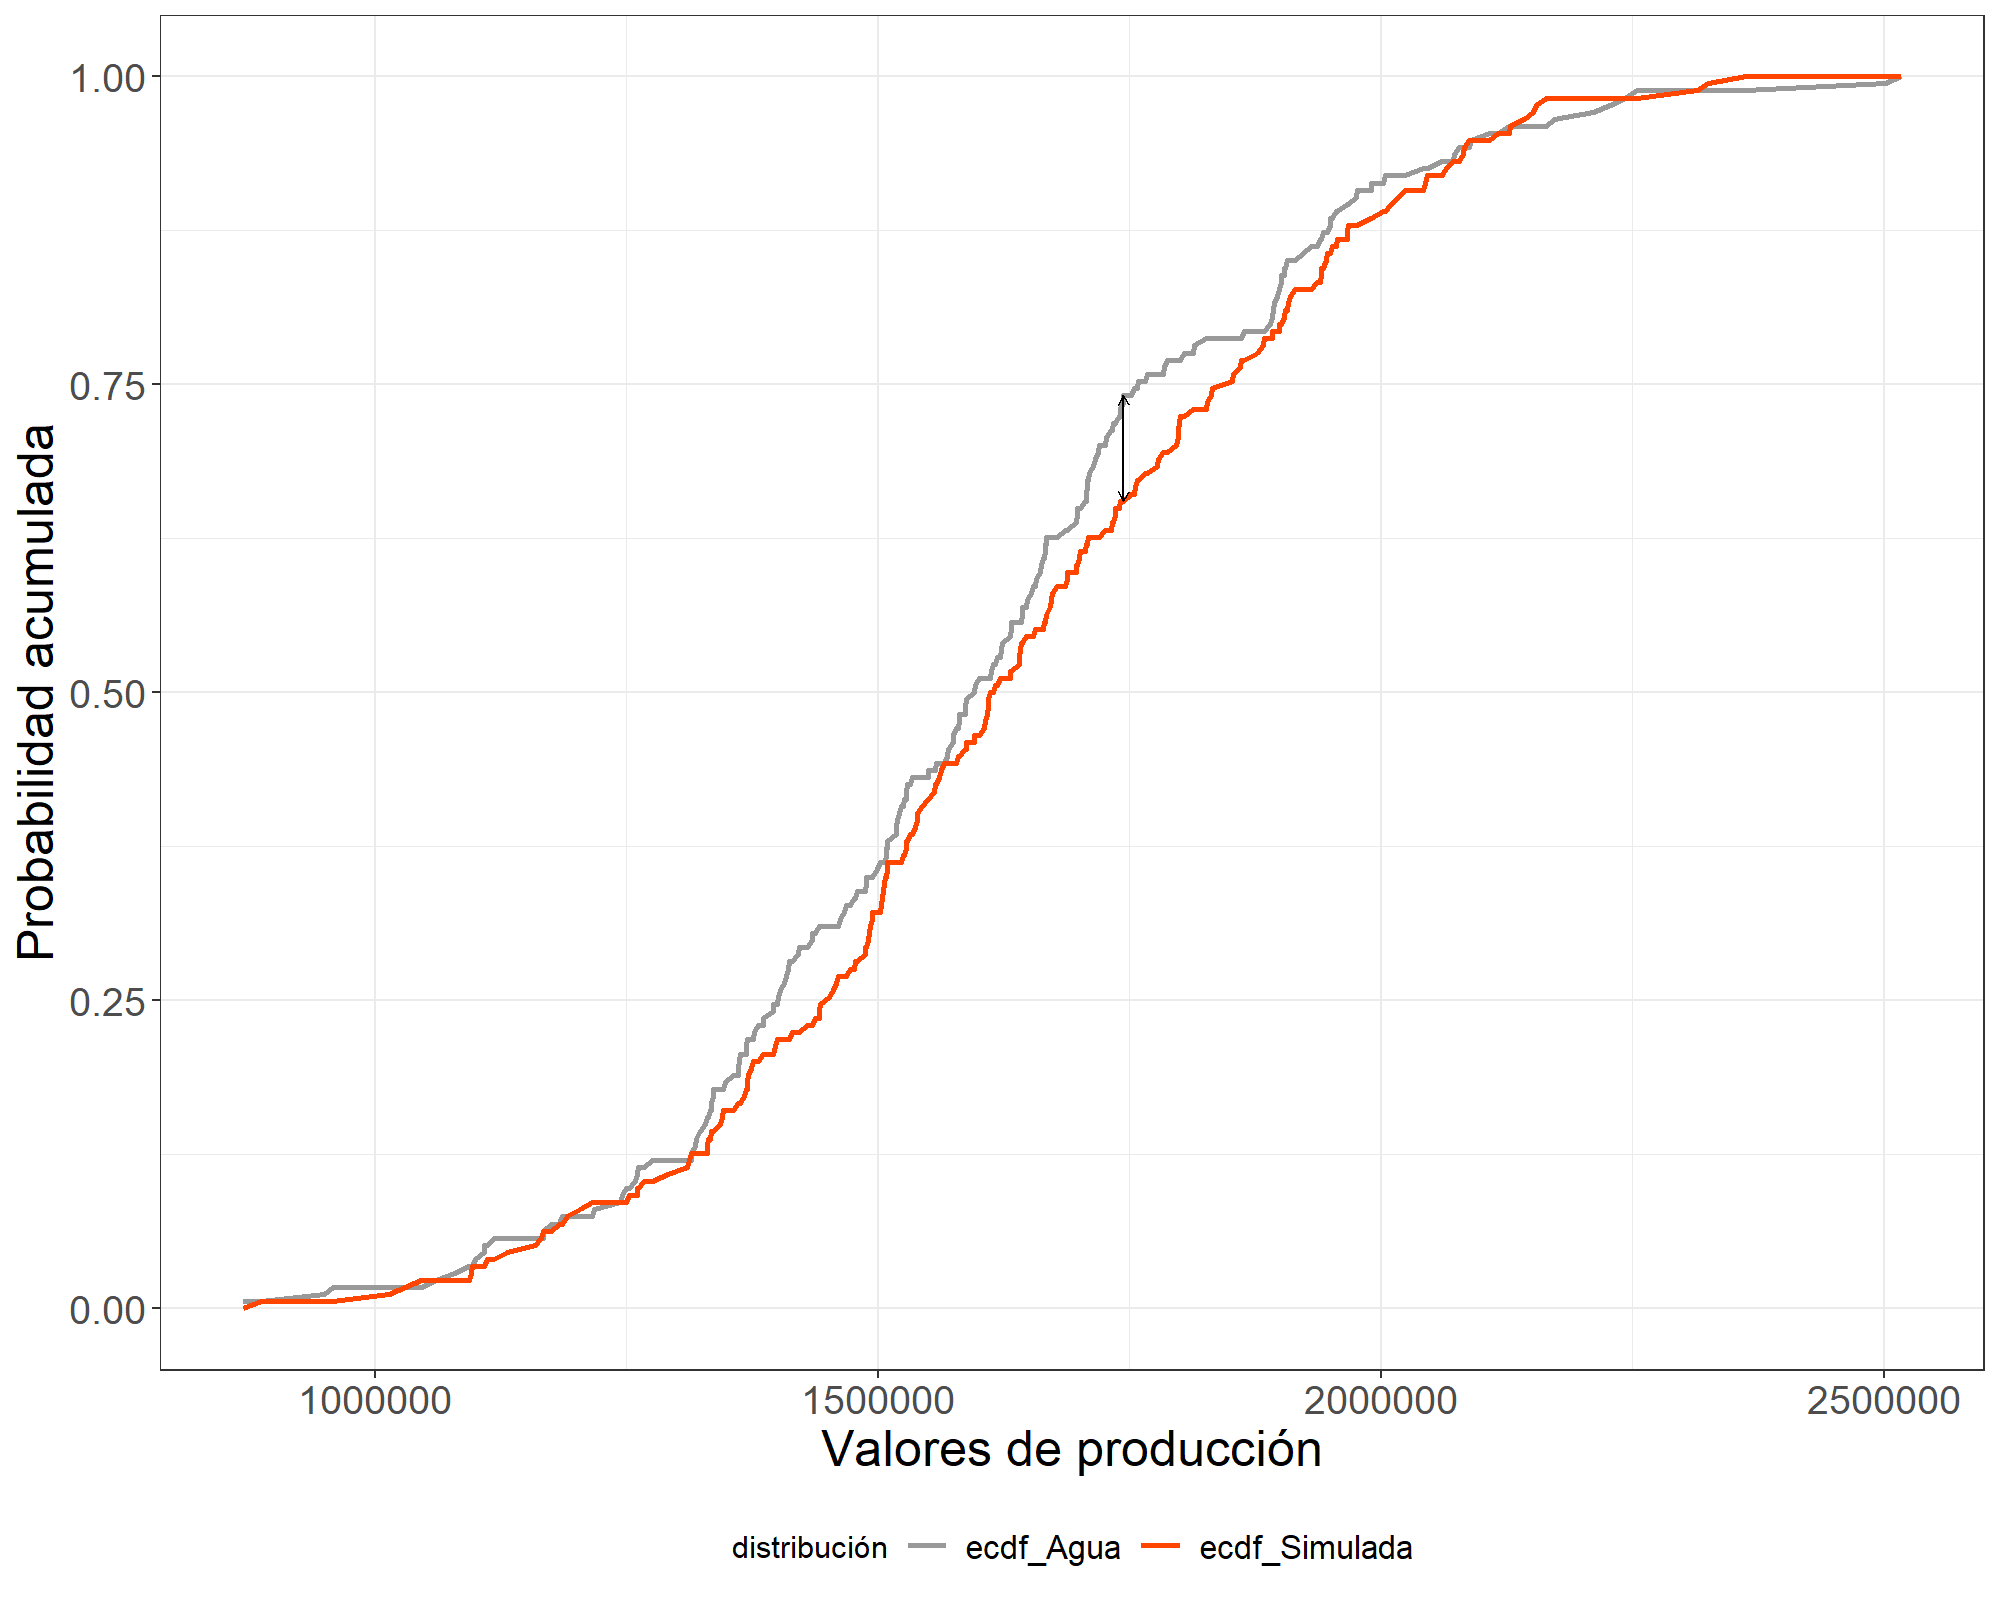
\includegraphics[scale=0.47]{figuras/DifSM.png}}
\label{fig:d}
\centering

\caption{Prueba de Kolmogorov-Smirnov }
\label{fig:10} 
\end{figure}
\subsection{Prueba F de Fisher}
La prueba F de Fisher se puede utilizar para comprobar que dos muestras tienen la misma varianza.

Para esta prueba se utilizan los datos pertenecientes al tipo de obra Agua, riego y saneamiento y datos creados con la función \textit{rnorm} de R. Con el objetivo de verificar si ambos poseen la misma varianza. La prueba se realiza con un $\alpha$ = 0.05, y la hipótesis planteada es la siguiente:
\begin{equation}\label{eq:1}
H_{0}:\text{(la varianza de Agua, riego y saneamiento)} = \text{(la varianza \textit{rnorm})}, 
\end{equation}
\begin{equation}\label{eq:2}
H_{1}: \text{(la varianza de Agua, riego y saneamiento)} \neq \text{(la varianza \textit{rnorm})}. 
\end{equation}
Los resultados obtenidos en la prueba, con un estadístico  \textbf{f} = 1.0442 y un \textbf{valor p} = 0.7766 mayor que $\alpha$, se puede concluir que no hay evidencias para rechazar la hipótesis $H_{0}$, por lo tanto los valores de producción de  tipo de obra Agua, riego y saneamiento y los valores creados con \textit{rnorm} tiene la misma varianza como era de esperarse, con un intervalo de confianza de 95\%.

\subsection{Prueba de Chi-cuadrada}
La prueba de chi-cuadrado en R se puede utilizar para probar si dos variables son dependientes.

Para esta prueba se utilizan los datos pertenecientes al tipo de obra Agua, riego y saneamiento. Con el objetivo de verificar estos son independientes con respecto al periodo en que fueron registrados. La prueba se realiza con un $\alpha$ = 0.05. Los resultados obtenidos en la prueba, con un estadístico  \textbf{$X^{2}$} = 2088 y un \textbf{valor p} = 0.4222 mayor que $\alpha$, se puede concluir que no hay evidencias para rechazar la hipótesis $H_{0}$, por lo tanto los valores de producción de  tipo de obra Agua, riego y saneamiento son valores independientes con respecto al periodo en que fueron registrados,con un intervalo de confianza de 95\%.

\subsection{Correlación}
La correlación nos indica la relación lineal de dos variables continuas.

Para esta prueba se utilizan los datos pertenecientes al tipo de obra Petróleo y petroquímica y Otras construcciones. La prueba se realiza con un $\alpha$ = 0.05.Los resultados obtenidos en la prueba, con un estadístico  \textbf{t} = 2.4082 y un \textbf{valor p} = 0.05709 mayor que $\alpha$, se puede concluir que no hay evidencias para rechazar la hipótesis $H_{0}$, por lo la correlación es cero,con un intervalo de confianza de 95\%.


El código general se encuentra disponible en el repositorio. \href{https://github.com/Albertomnoa/Tareas_MPA/tree/master/Tarea4}{https://github.com/Albertomnoa/Tareas} 

\newpage
\bibliographystyle{plain}
\bibliography{Biblio}

\end{document}
